\section{Results}\label{section:star_results}

\begin{figure}[bh]
	\centering
	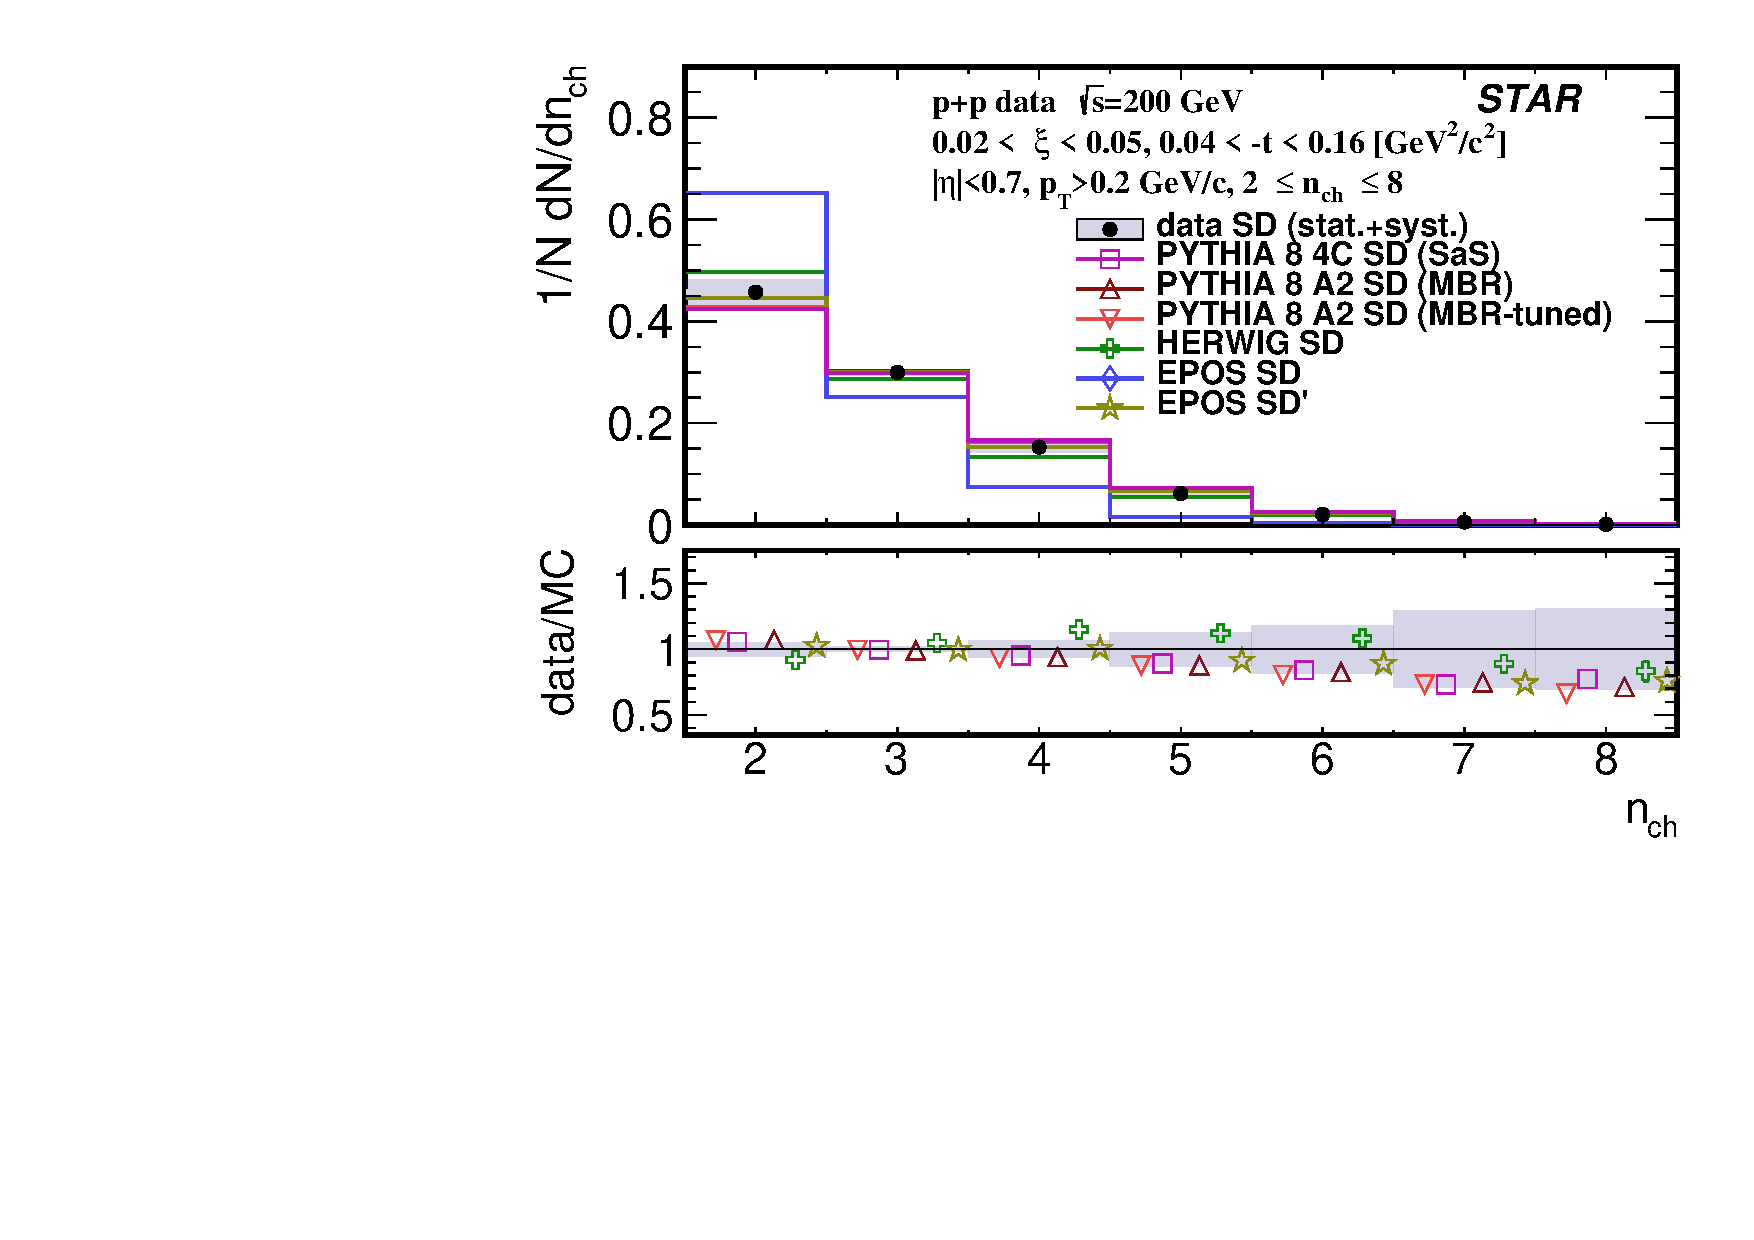
\includegraphics[width=.49\textwidth,page=1]{chapters/chrgSTAR/img/results/nch_ksi_0.pdf}
	\hfill
	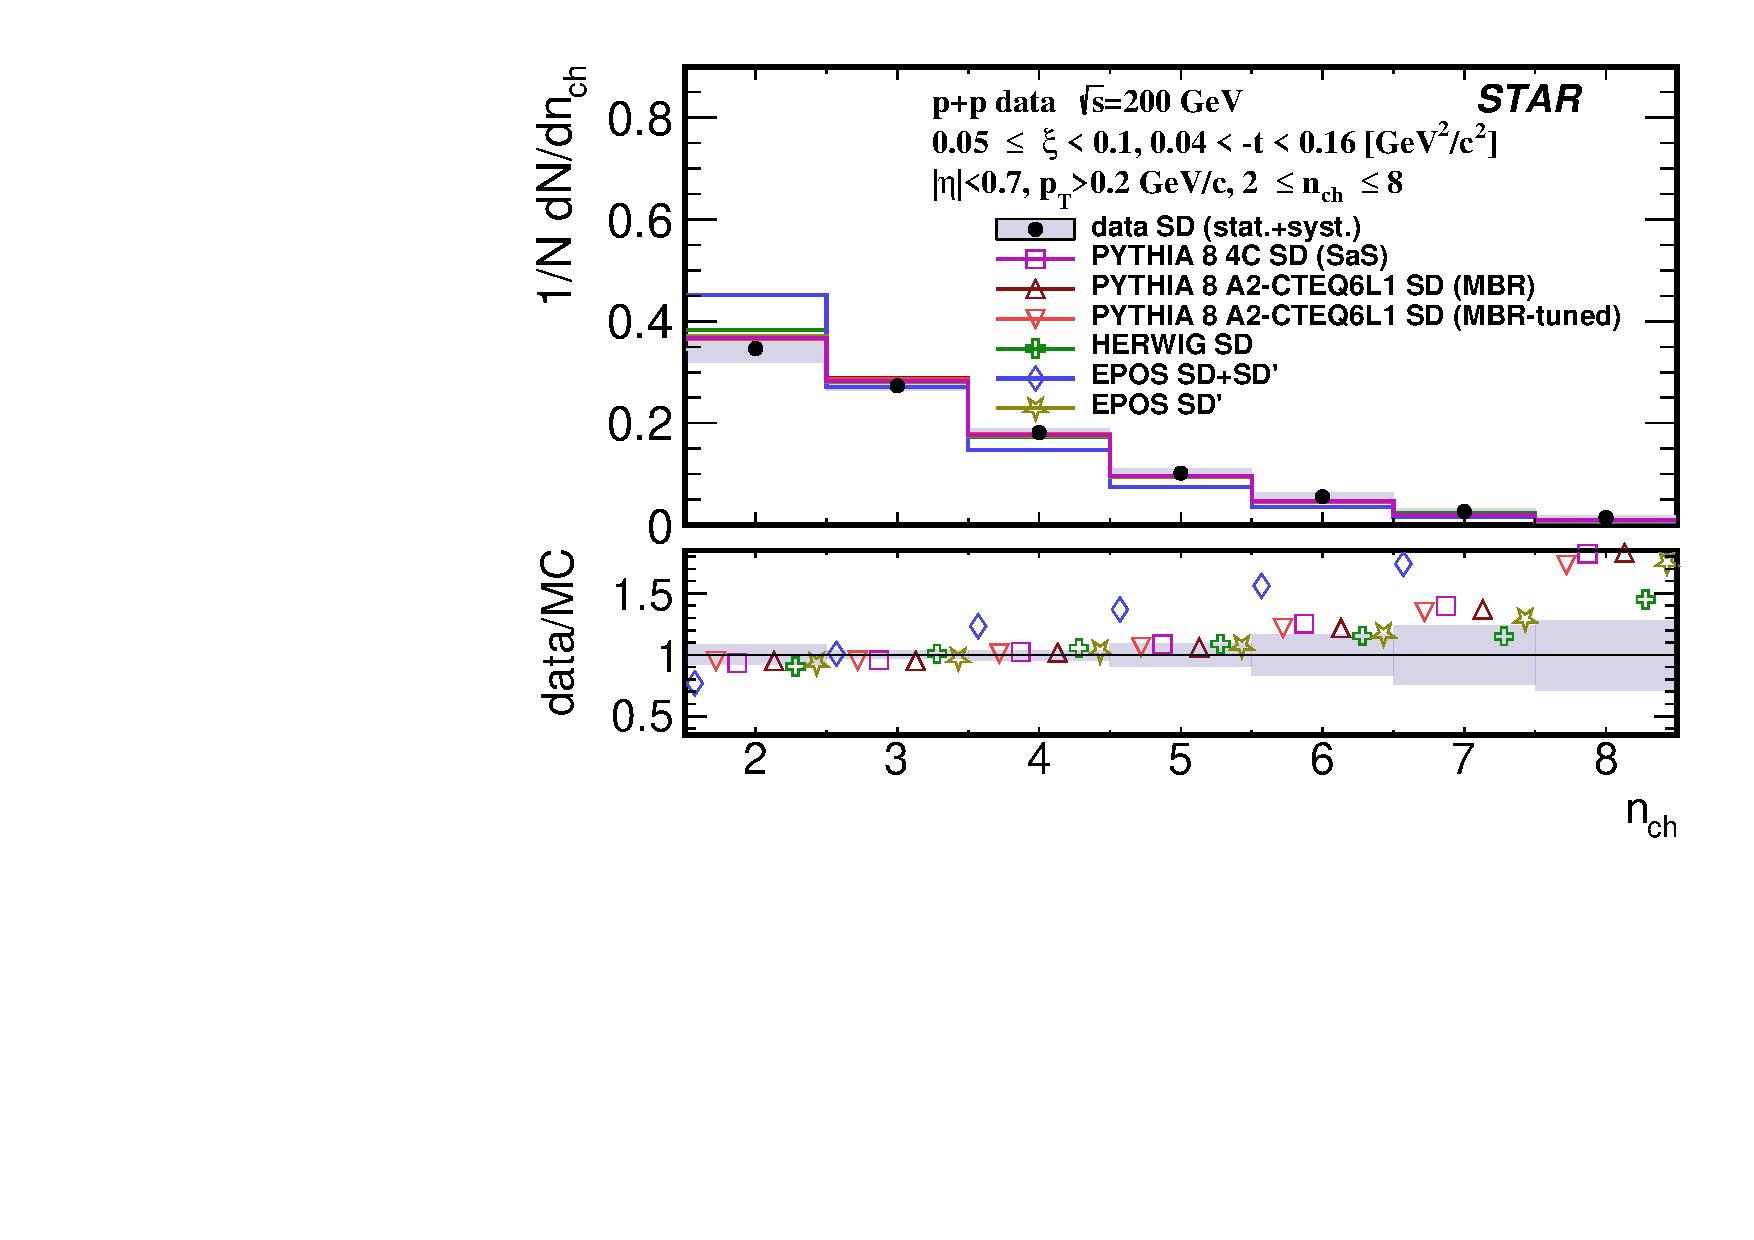
\includegraphics[width=.49\textwidth,page=1]{chapters/chrgSTAR/img/results/nch_ksi_1.pdf}
	\newline
	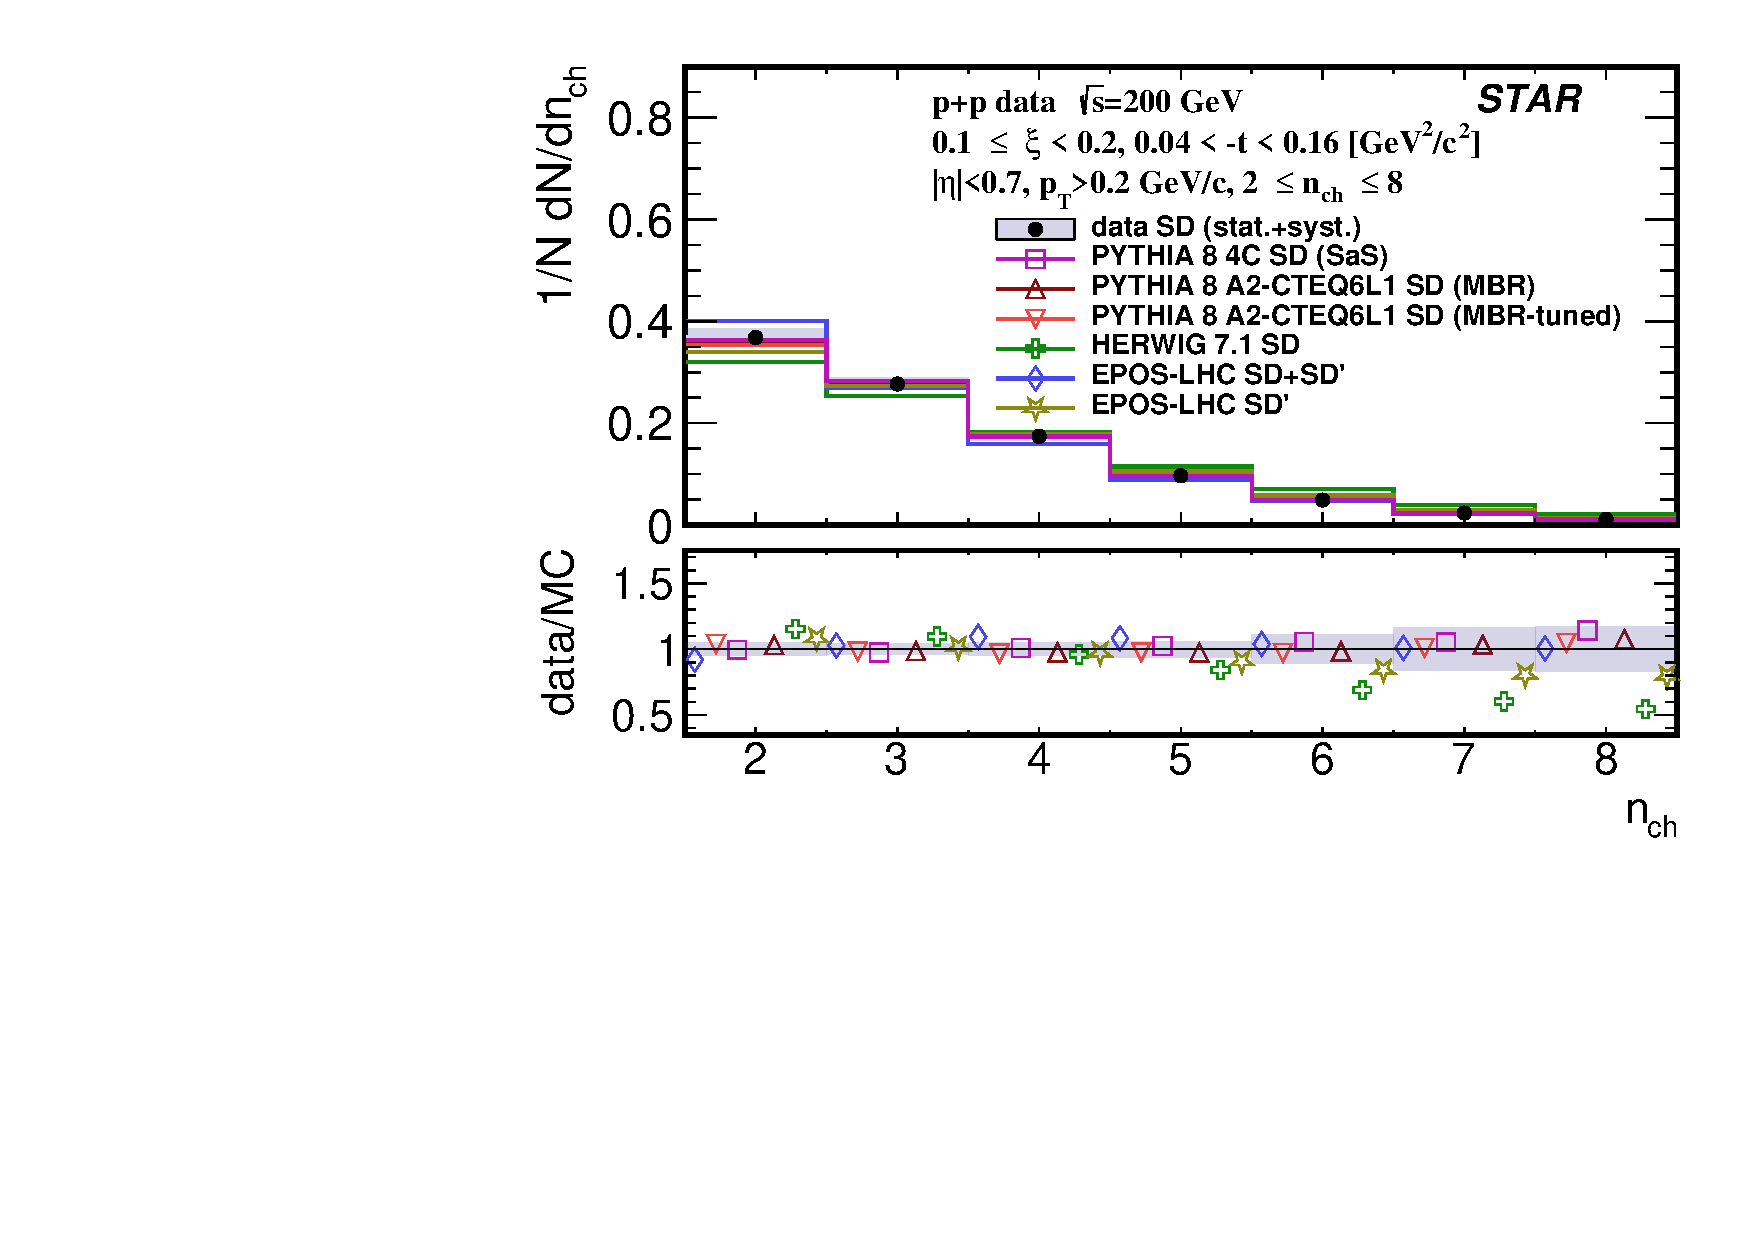
\includegraphics[width=.49\textwidth,page=1]{chapters/chrgSTAR/img/results/nch_ksi_2.pdf}
	\hfill
	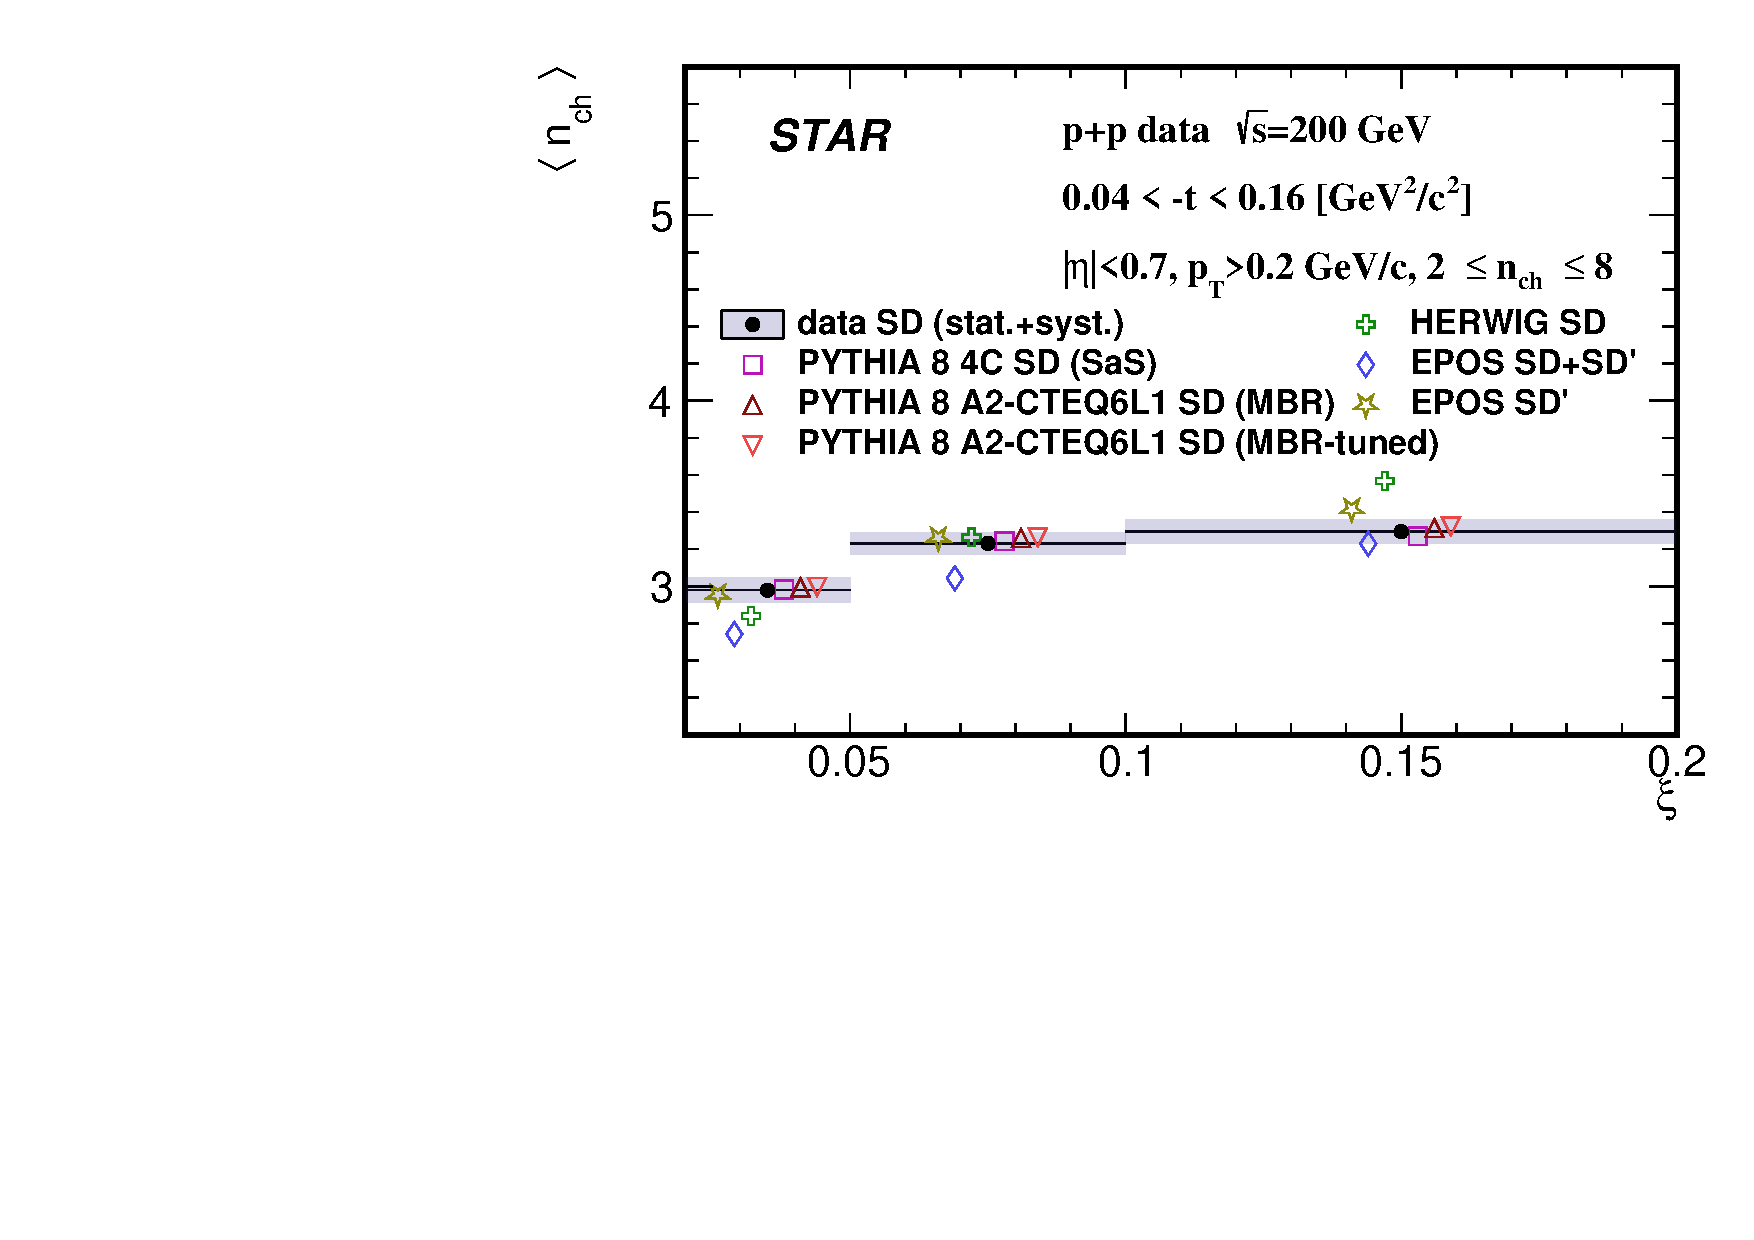
\includegraphics[width=.49\textwidth,page=1]{chapters/chrgSTAR/img/results/mean_nch_xi.pdf}
	%
	\caption[Primary charged-particle multiplicity shown separately for three ranges of the $\xi$  and the mean multiplicity $\langle n_{ch}\rangle$ as a function of $\xi$.]{Primary charged-particle multiplicity shown separately for three ranges of the $\xi$: (top left) $0.02<\xi<0.05$, (top right) $0.05<\xi<0.1$, (bottom left) $0.1<\xi<0.2$ and (bottom right) the mean multiplicity $\langle n_{ch}\rangle$ as a function of $\xi$.}
	\label{results_star_nch}
\end{figure}

\begin{figure}[bh]
	\centering
	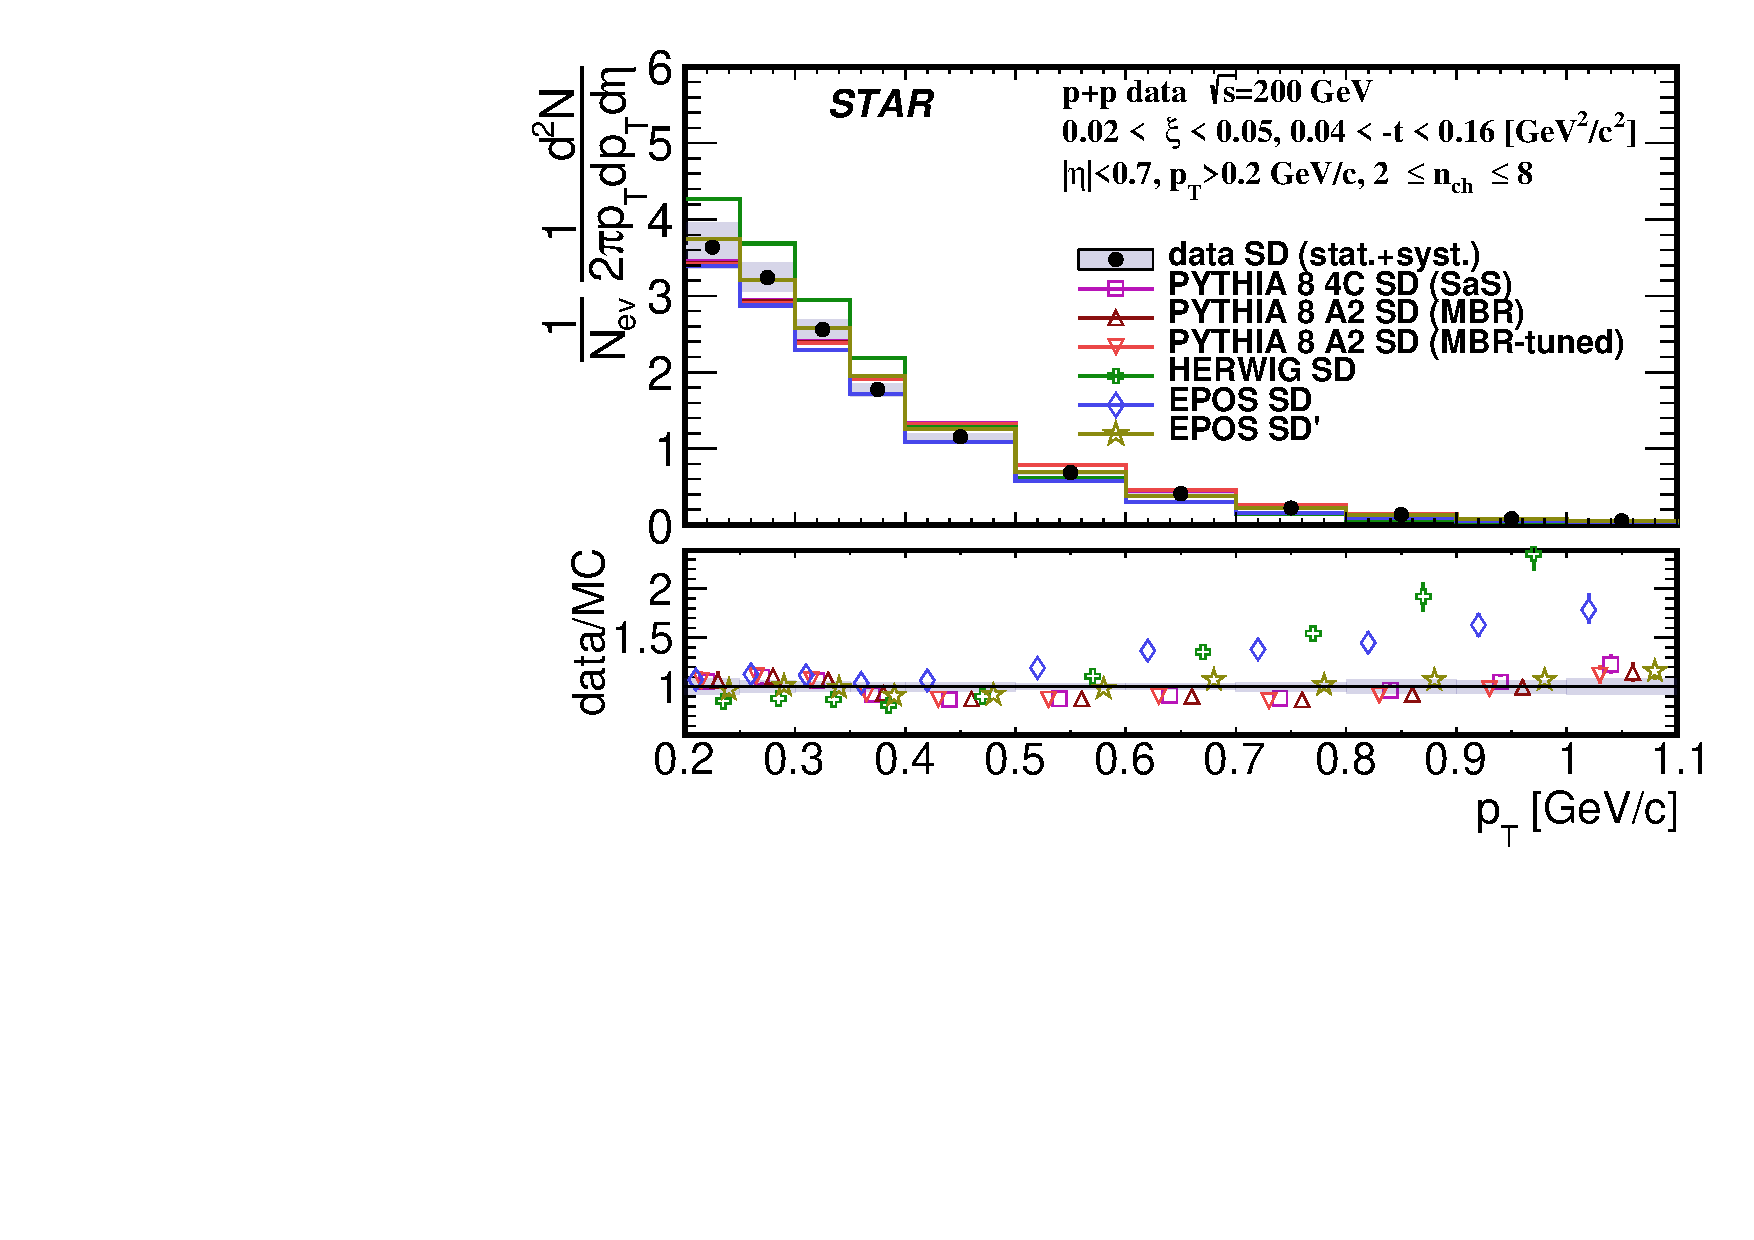
\includegraphics[width=.49\textwidth,page=1]{chapters/chrgSTAR/img/results/out_pt_ksi_0.pdf}
	\hfill
	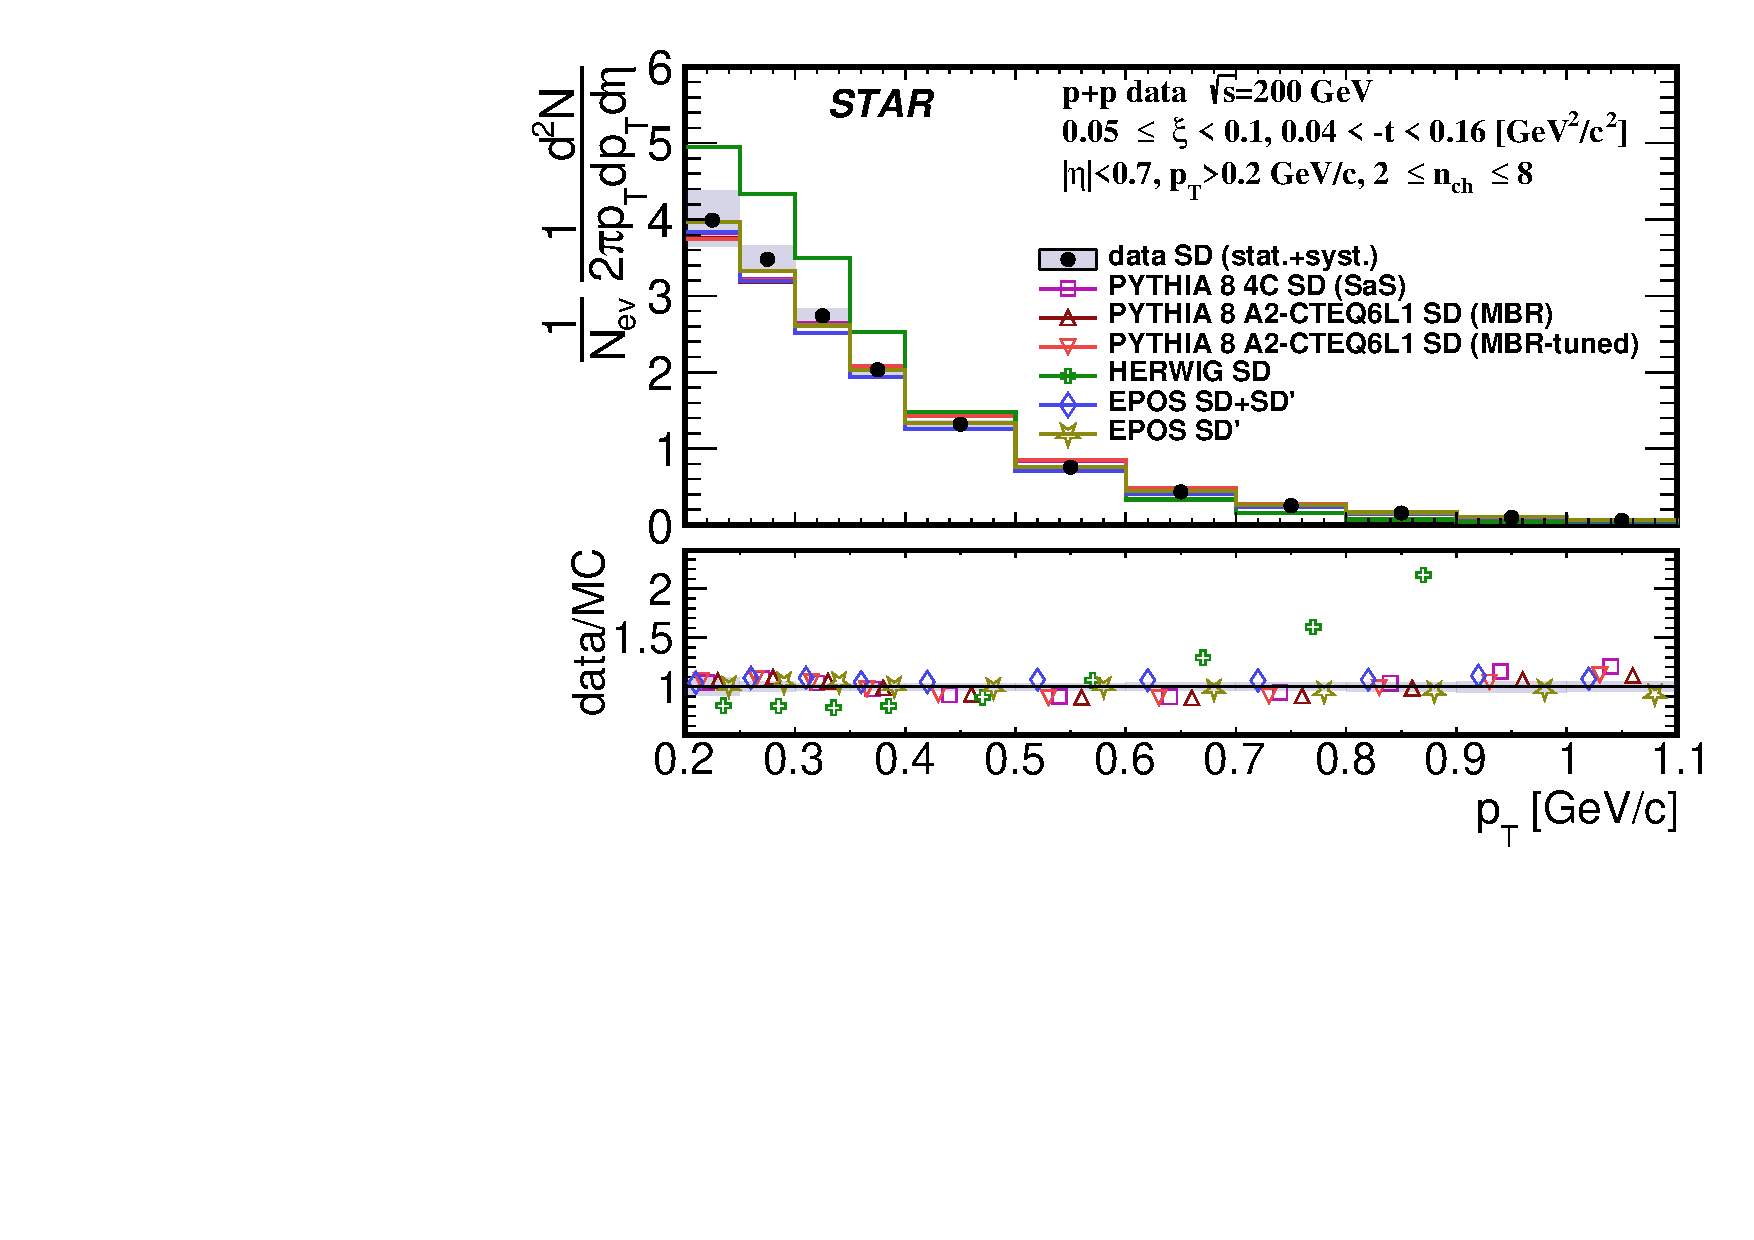
\includegraphics[width=.49\textwidth,page=1]{chapters/chrgSTAR/img/results/out_pt_ksi_1.pdf}
	\newline
	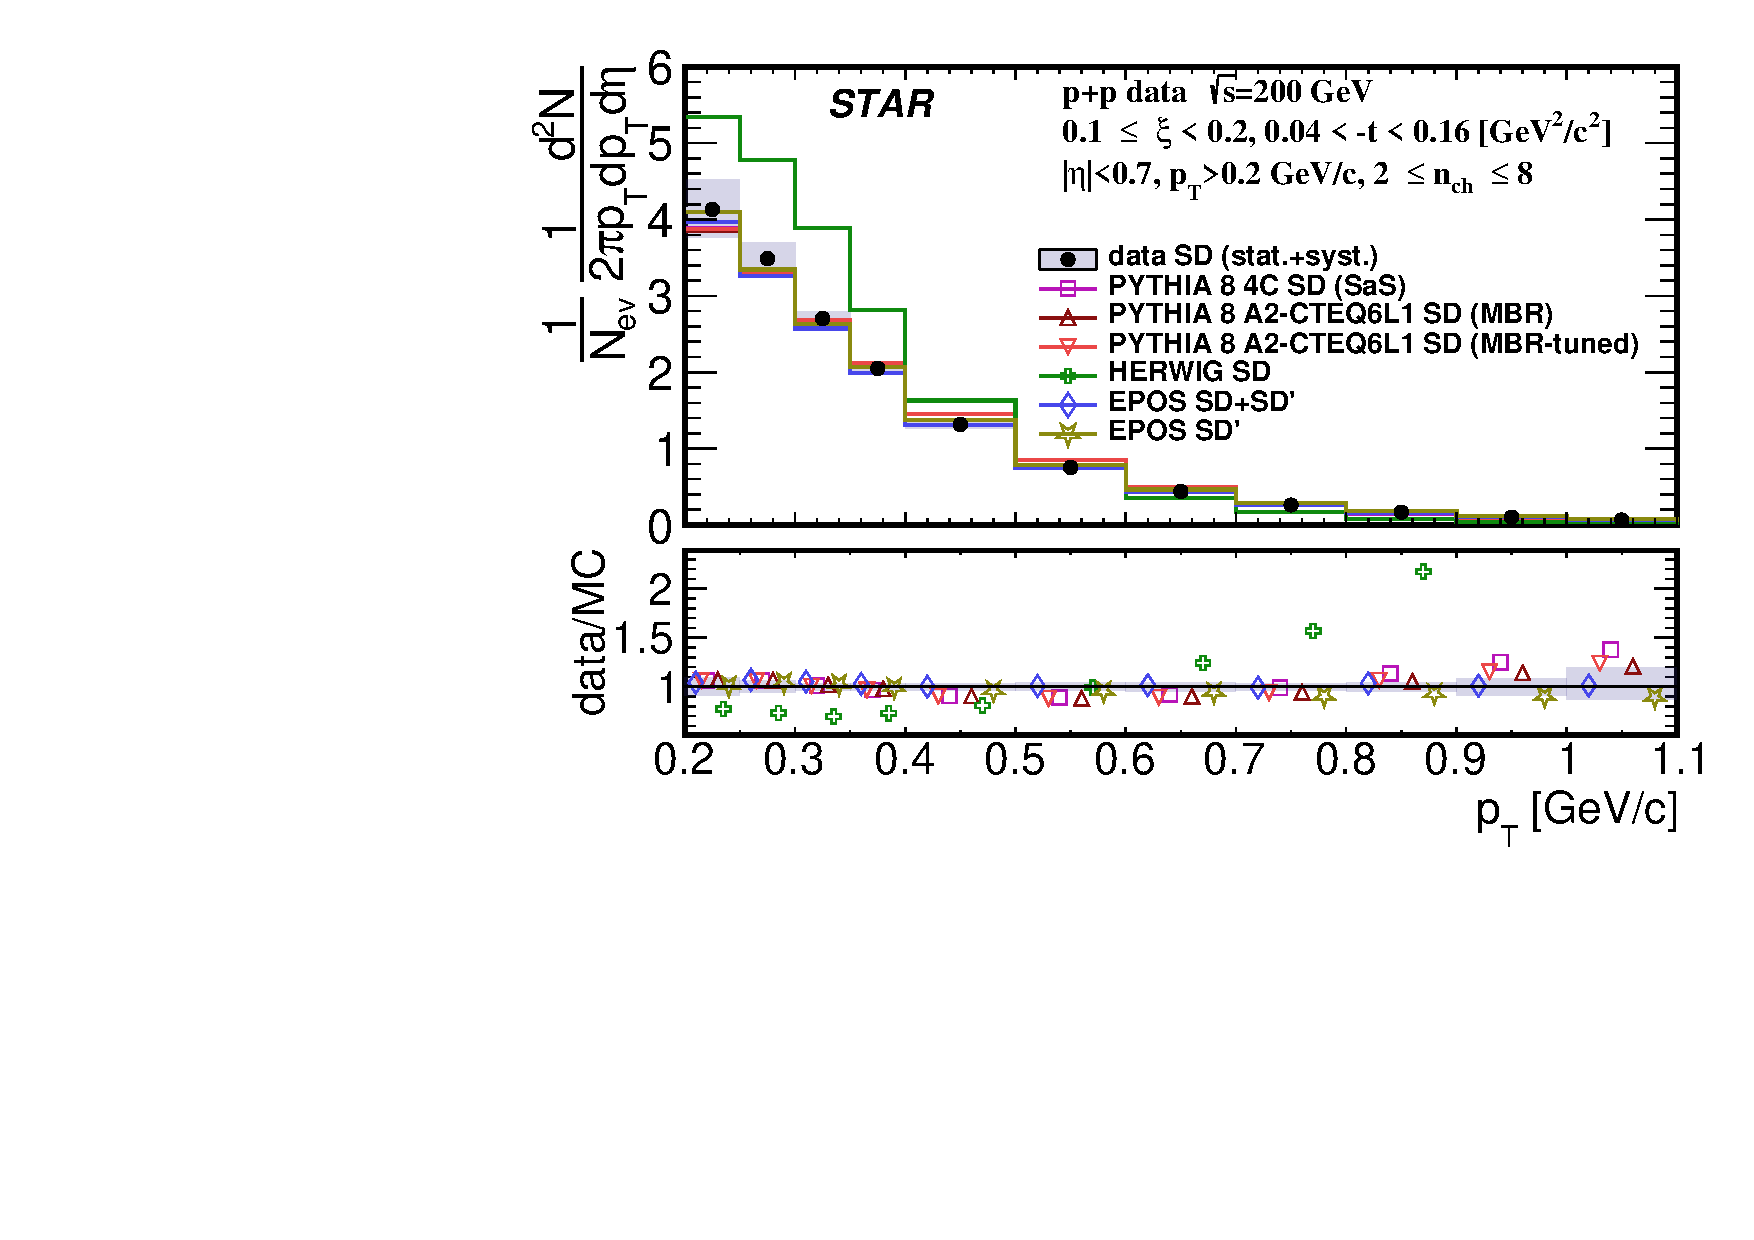
\includegraphics[width=.49\textwidth,page=1]{chapters/chrgSTAR/img/results/out_pt_ksi_2.pdf}
	\hfill
	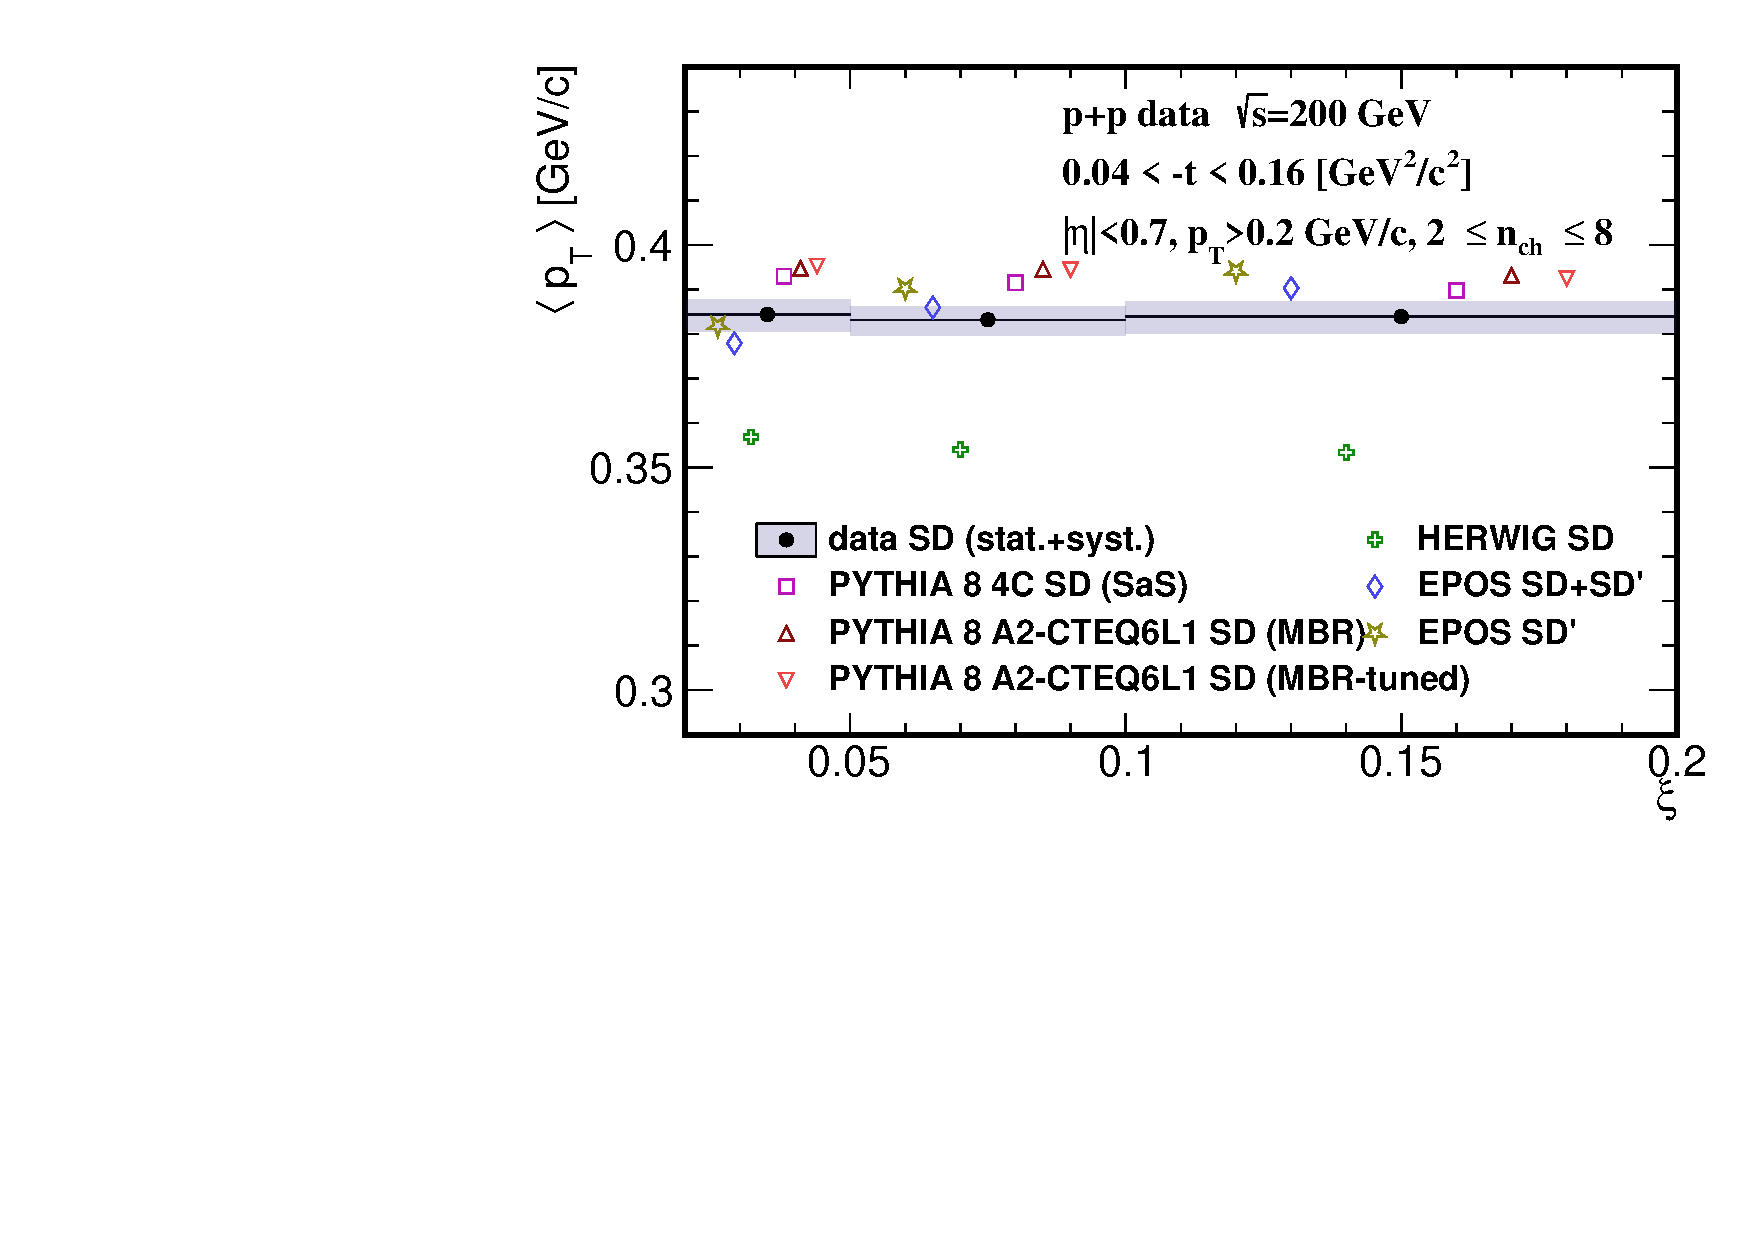
\includegraphics[width=.49\textwidth,page=1]{chapters/chrgSTAR/img/results/mean_pt_xi.pdf}
	%
	\caption[Primary charged-particle multiplicities as a function of $p_T$ shown separately for three ranges of the $\xi$ and the mean transverse momenta $\langle p_T\rangle$ as a function of $\xi$.]{Primary charged-particle multiplicities as a function of $p_T$ shown separately for three ranges of the $\xi$: (top left) $0.02<\xi<0.05$, (top right) $0.05<\xi<0.1$, (bottom left) $0.1<\xi<0.2$ and (bottom right) the mean transverse momenta $\langle p_T\rangle$ as a function of $\xi$.}
	\label{results_star_pt}
\end{figure}

\begin{figure}[bh]
	\centering
	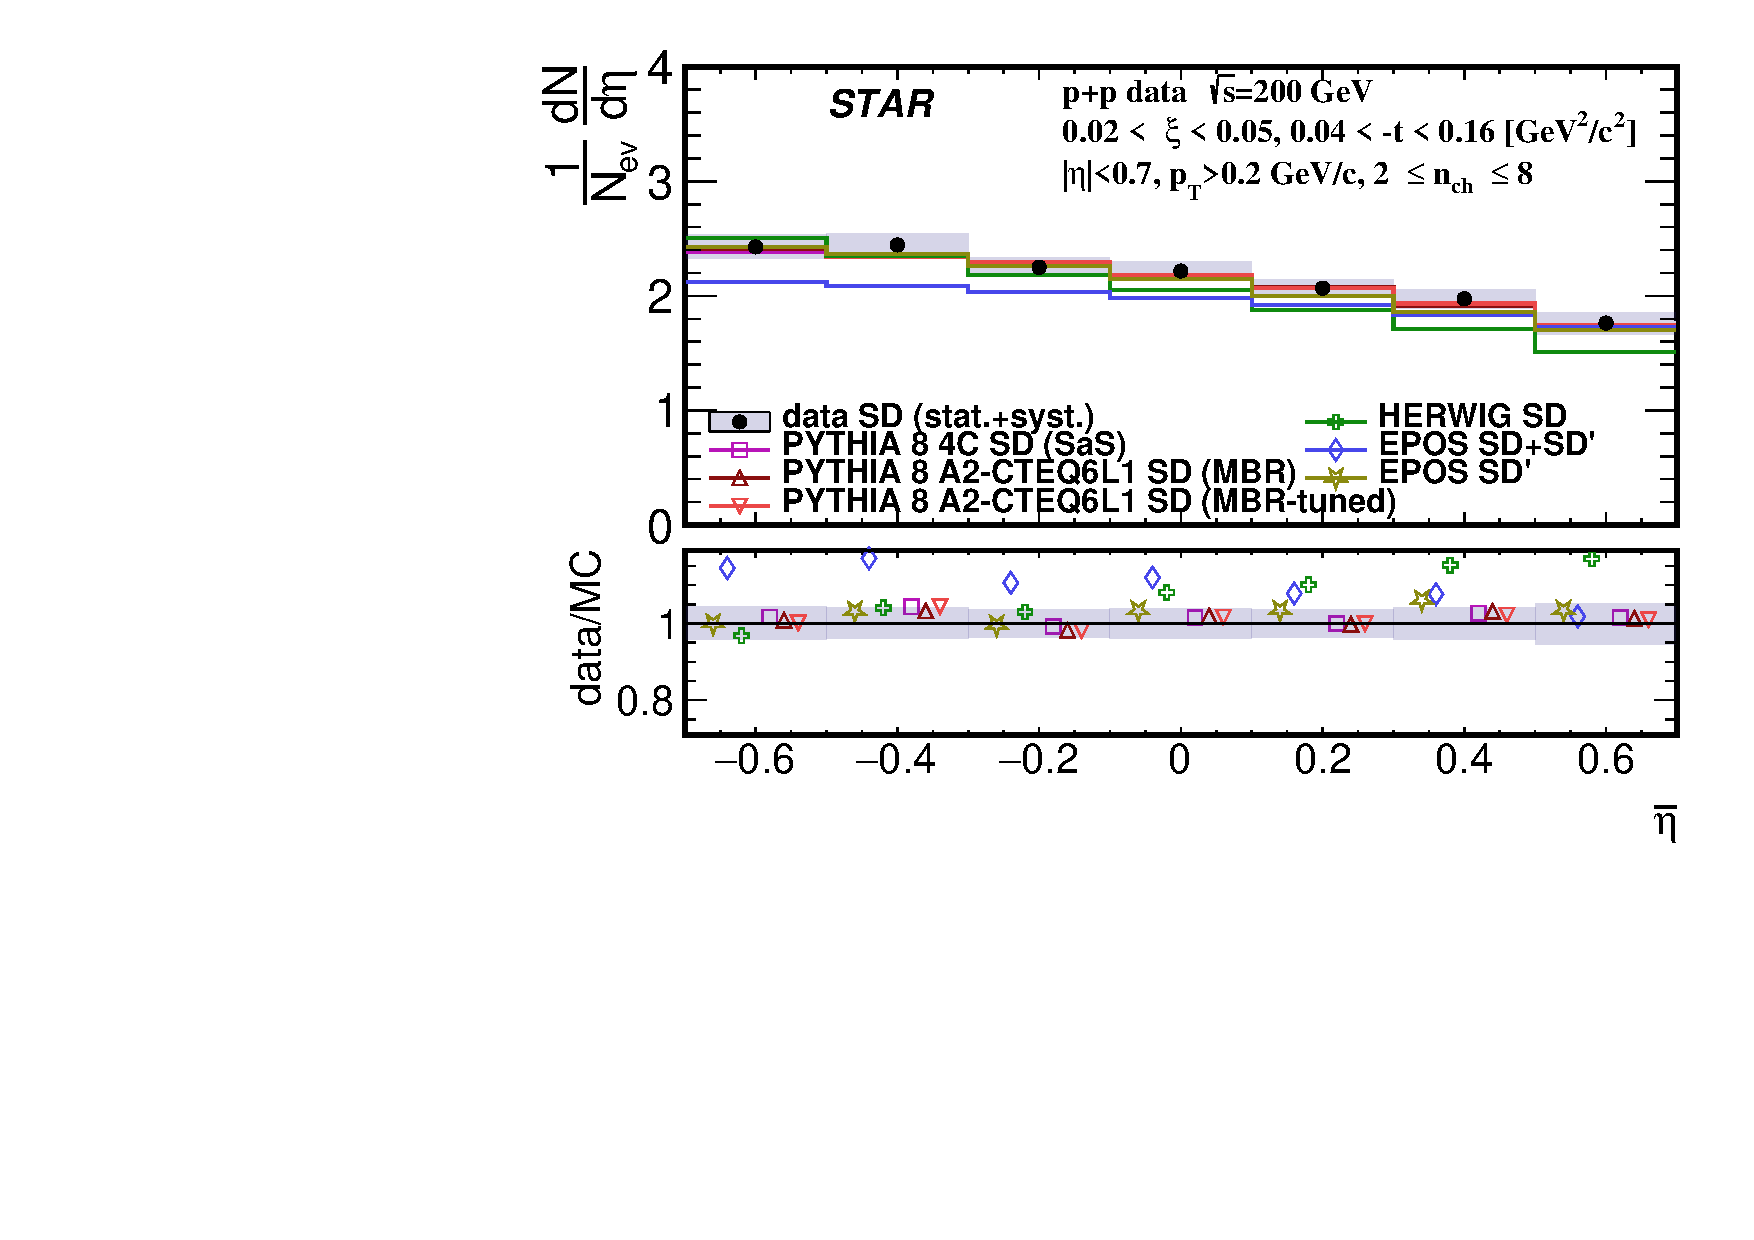
\includegraphics[width=.49\textwidth,page=1]{chapters/chrgSTAR/img/results/out_eta_SD_0.pdf}
	\hfill
	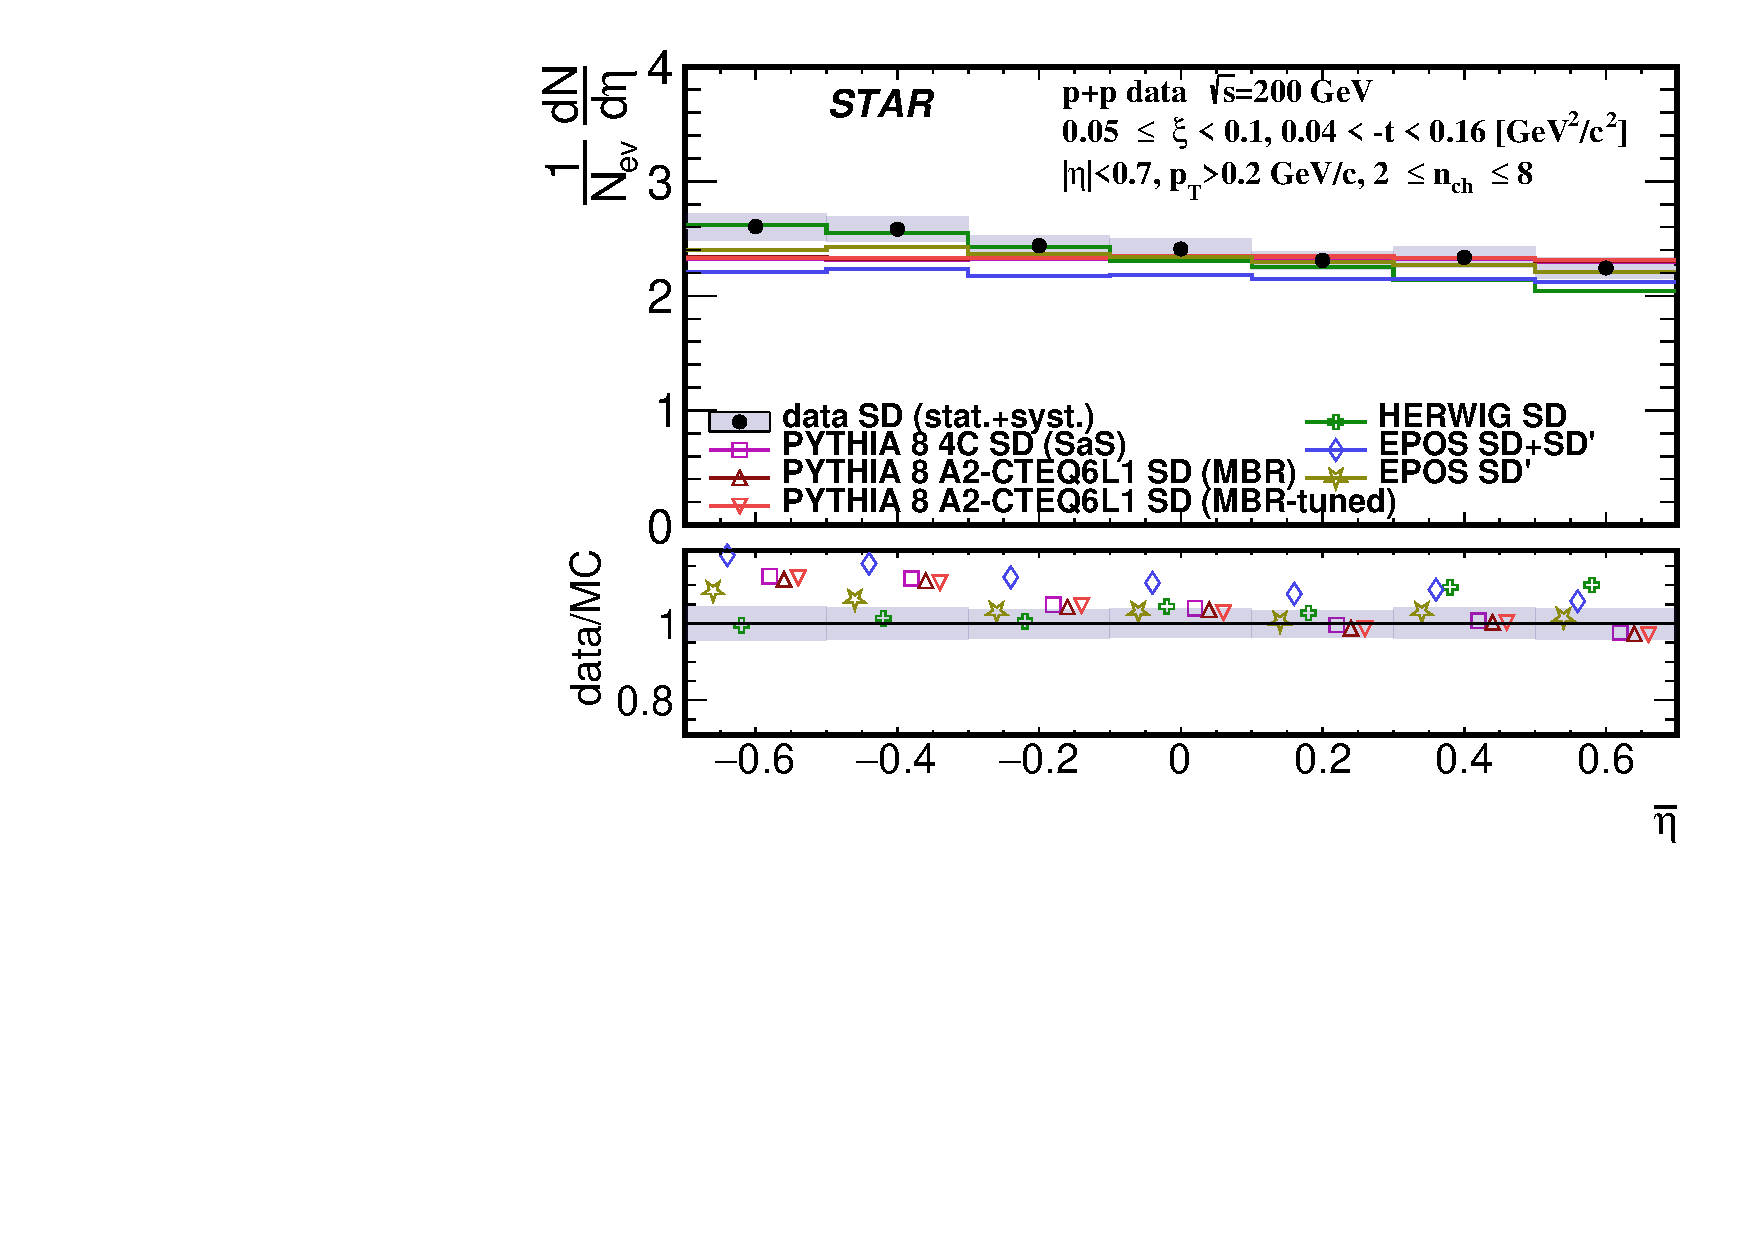
\includegraphics[width=.49\textwidth,page=1]{chapters/chrgSTAR/img/results/out_eta_SD_1.pdf}
	\newline
	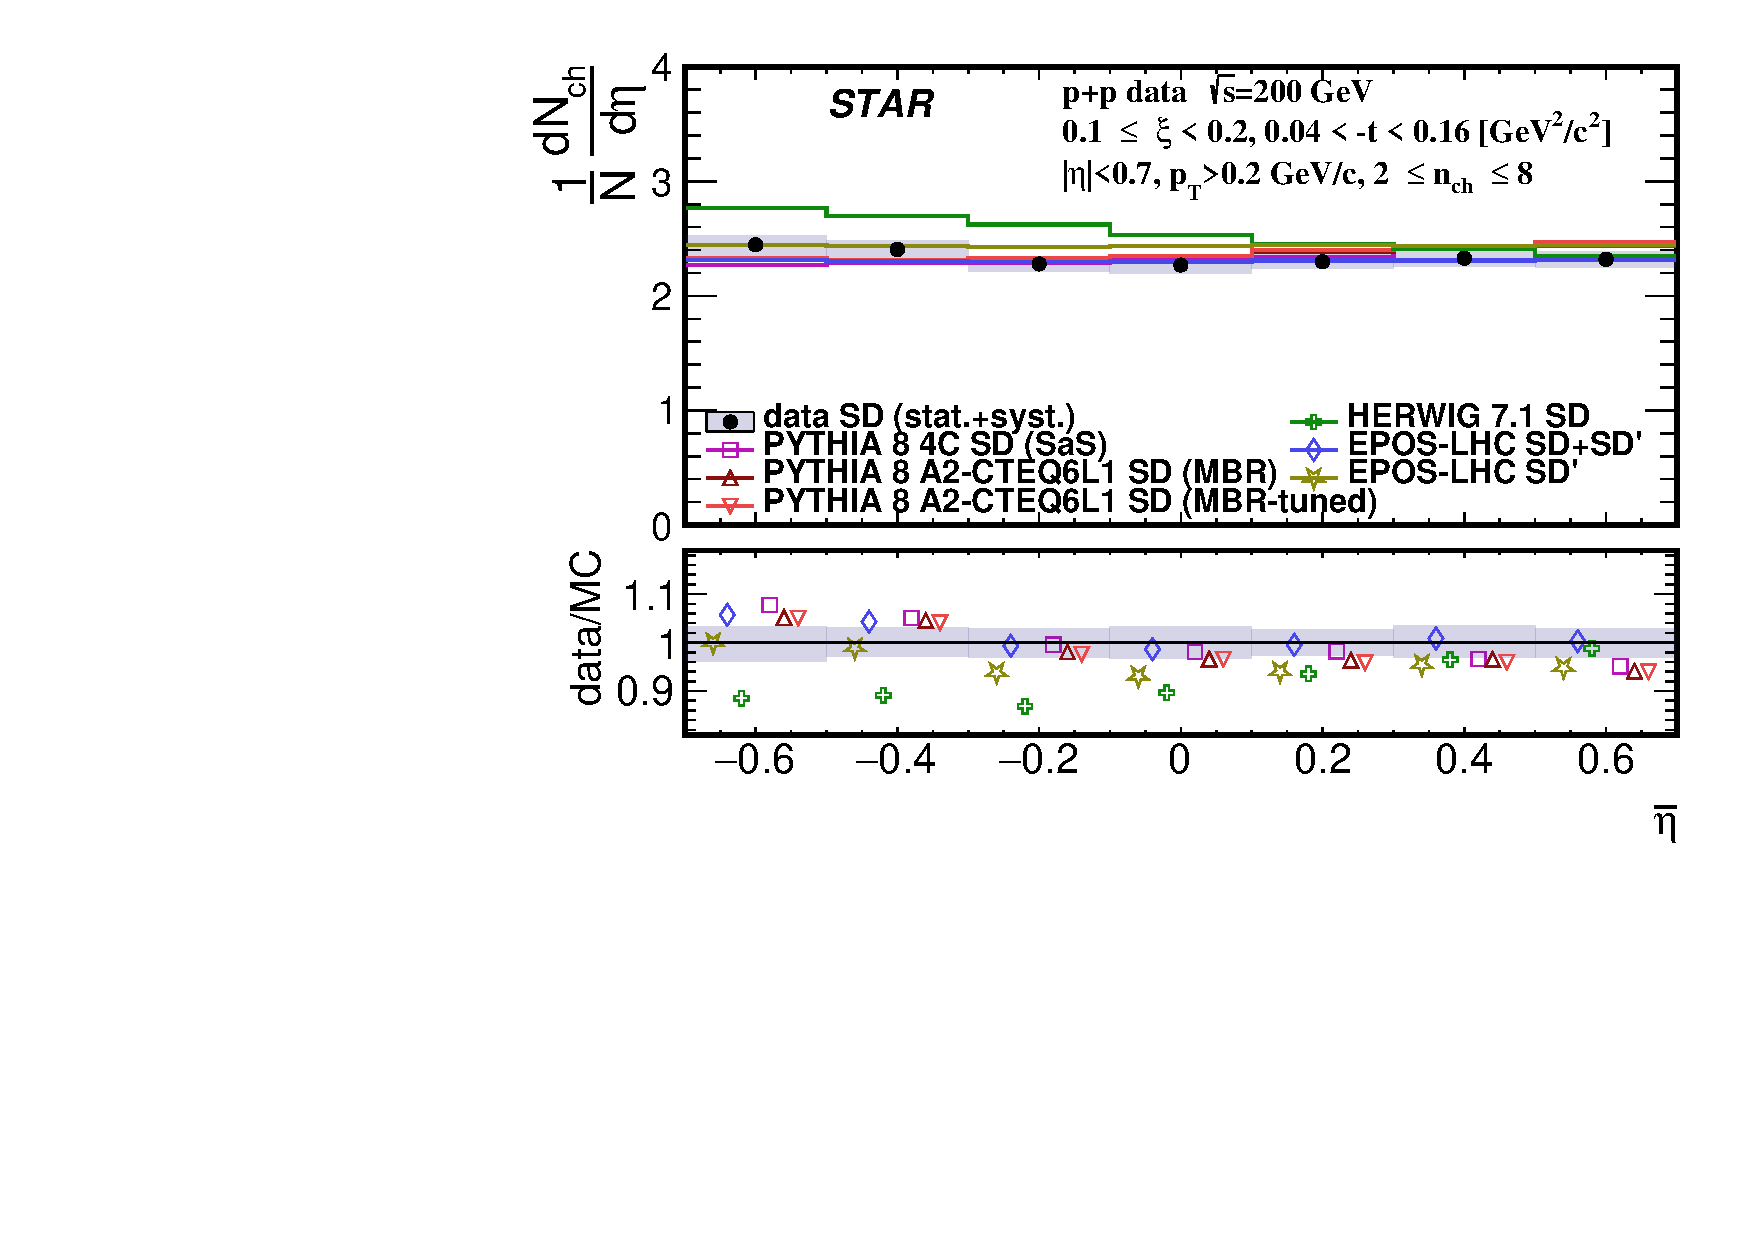
\includegraphics[width=.49\textwidth,page=1]{chapters/chrgSTAR/img/results/out_eta_SD_2.pdf}
	\hfill
	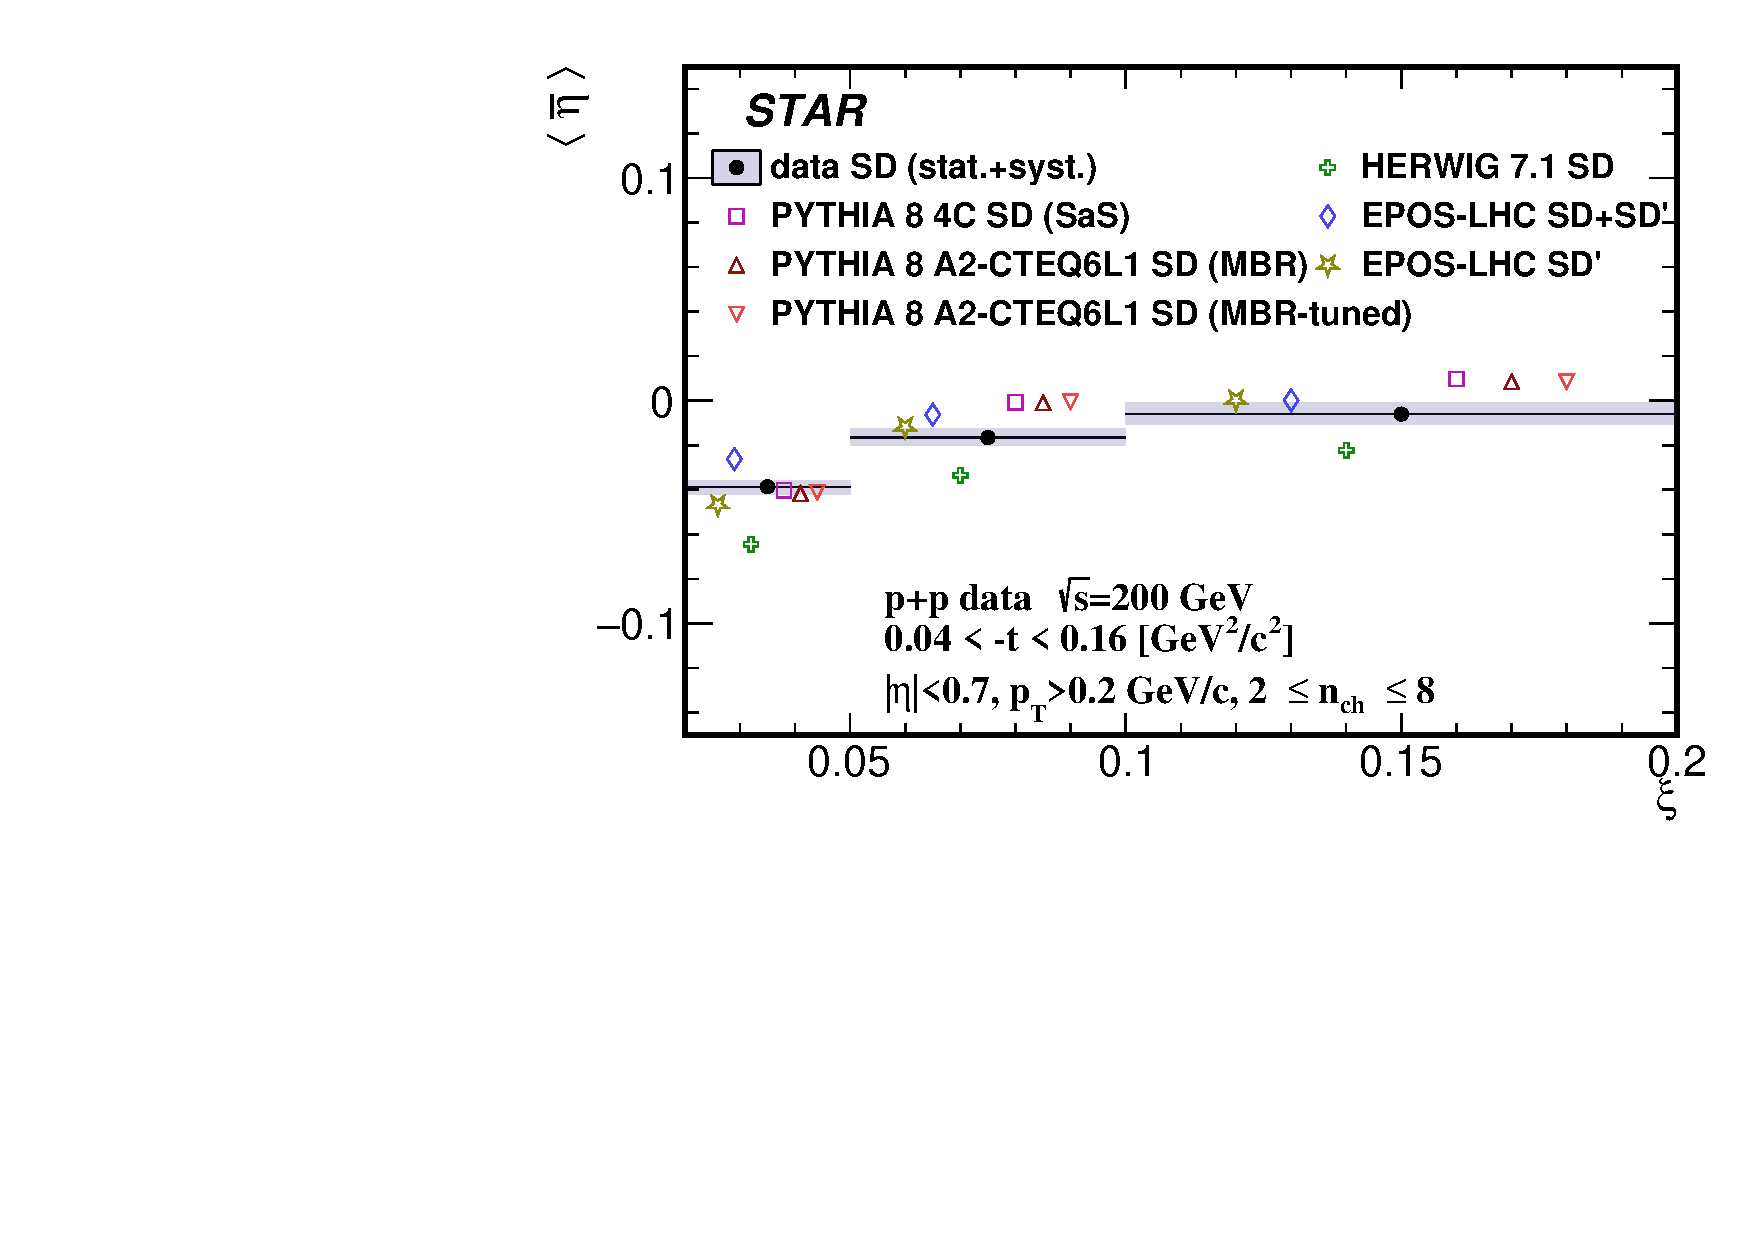
\includegraphics[width=.49\textwidth,page=1]{chapters/chrgSTAR/img/results/mean_eta_xi.pdf}
	%
	\caption[Primary charged-particle multiplicity as a function of $\bar{\eta}$ shown  separately for three ranges of the $\xi$ and the mean pseudorapidity  $\langle\bar{\eta}\rangle$ as a function of $\xi$.]{Primary charged-particle multiplicity as a function of $\bar{\eta}$ shown  separately for three ranges of the $\xi$: (top left) $0.02<\xi<0.05$, (top right) $0.05<\xi<0.1$, (bottom left) $0.1<\xi<0.2$ and (bottom right) the mean pseudorapidity  $\langle\bar{\eta}\rangle$ as a function of $\xi$.}
	\label{results_star_eta}
\end{figure}

\begin{figure}[bh]
	\centering
	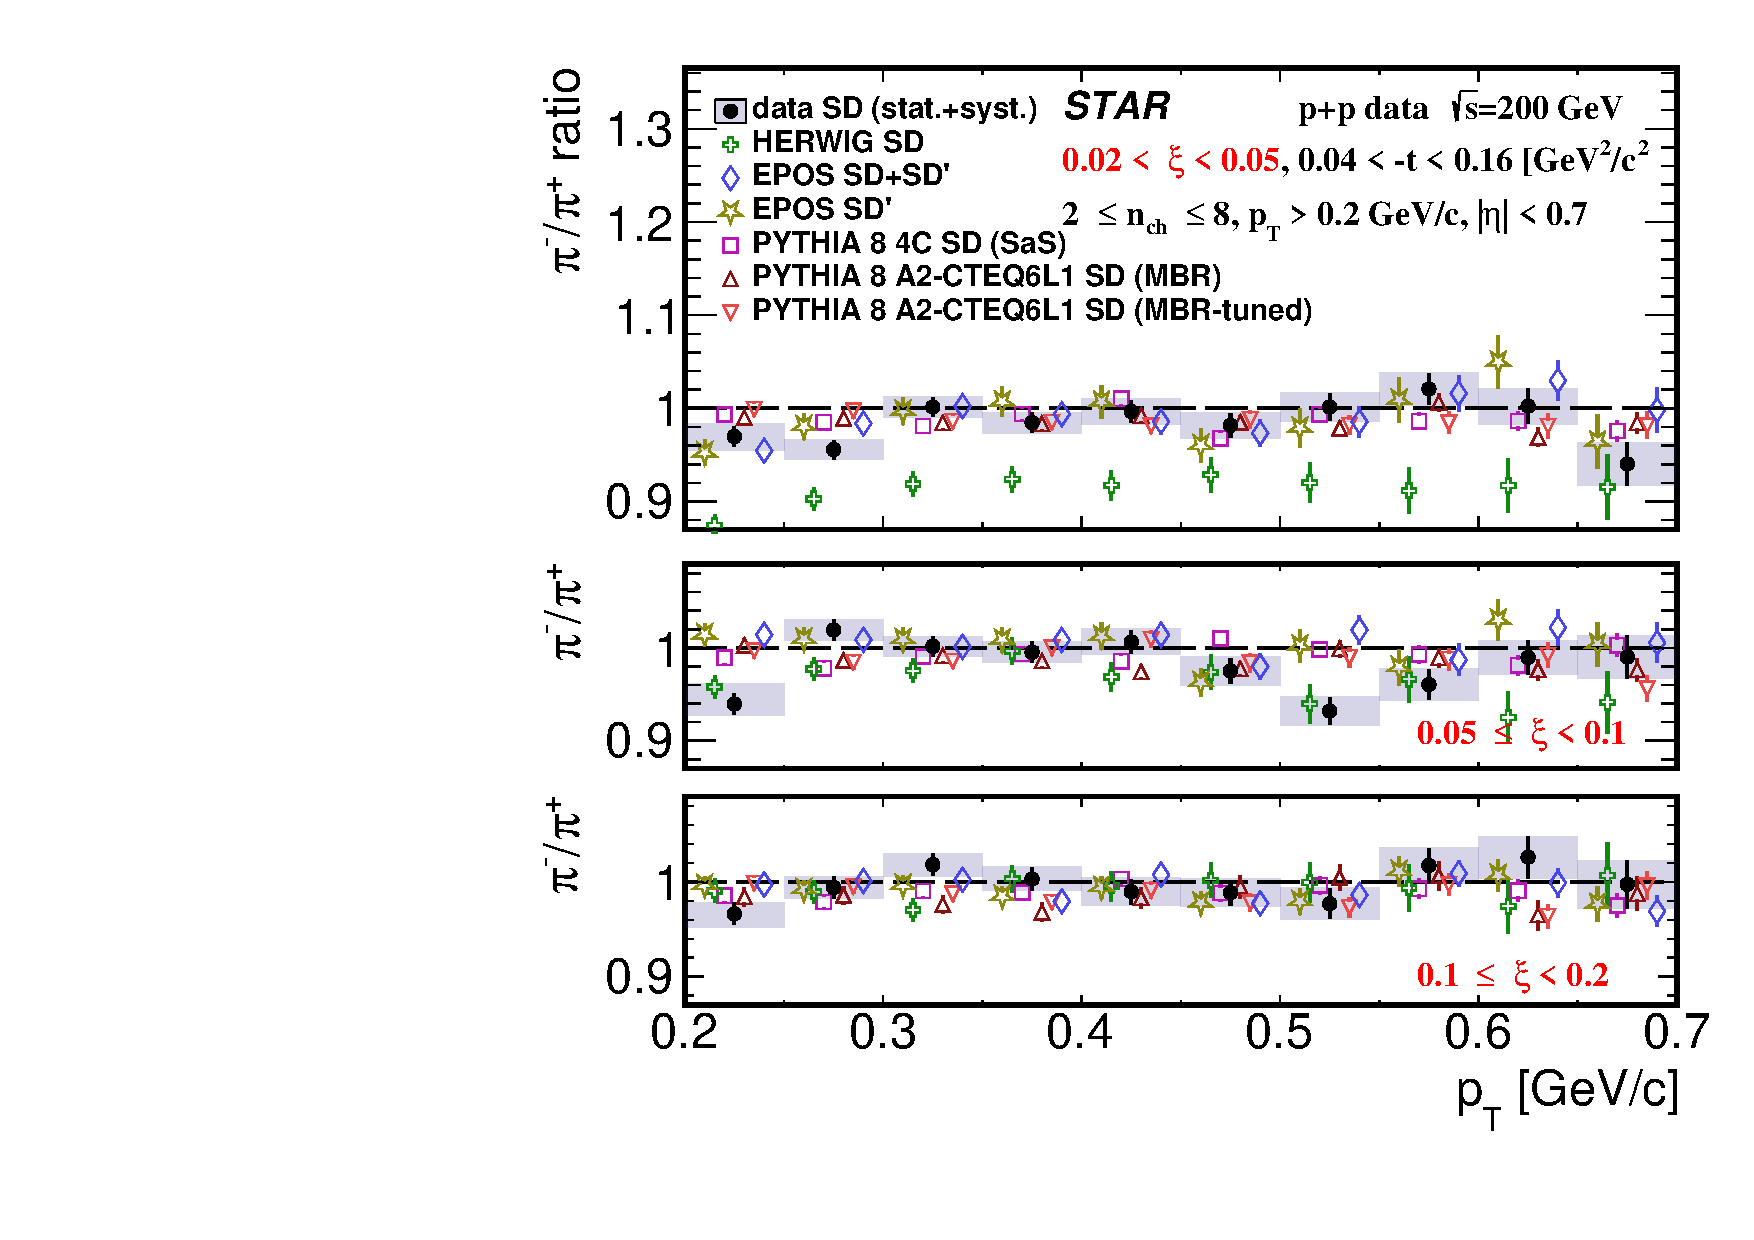
\includegraphics[width=.99\textwidth,page=1]{chapters/chrgSTAR/img/results/particleRatio_prt_0.pdf}
	%
	\caption[Ratio of production yields of $\pi^-/\pi^+$ as a function of $p_T$ shown separately for three ranges of the $\xi$.]{Ratio of production yields of $\pi^-/\pi^+$ as a function of $p_T$ shown separately for three ranges of the $\xi$: (top) $0.02<\xi<0.05$, (middle) $0.05<\xi<0.1$, (bottom) $0.1<\xi<0.2$.}
	\label{results_star_pion}
	
\end{figure}

\begin{figure}[bh]
	\centering
	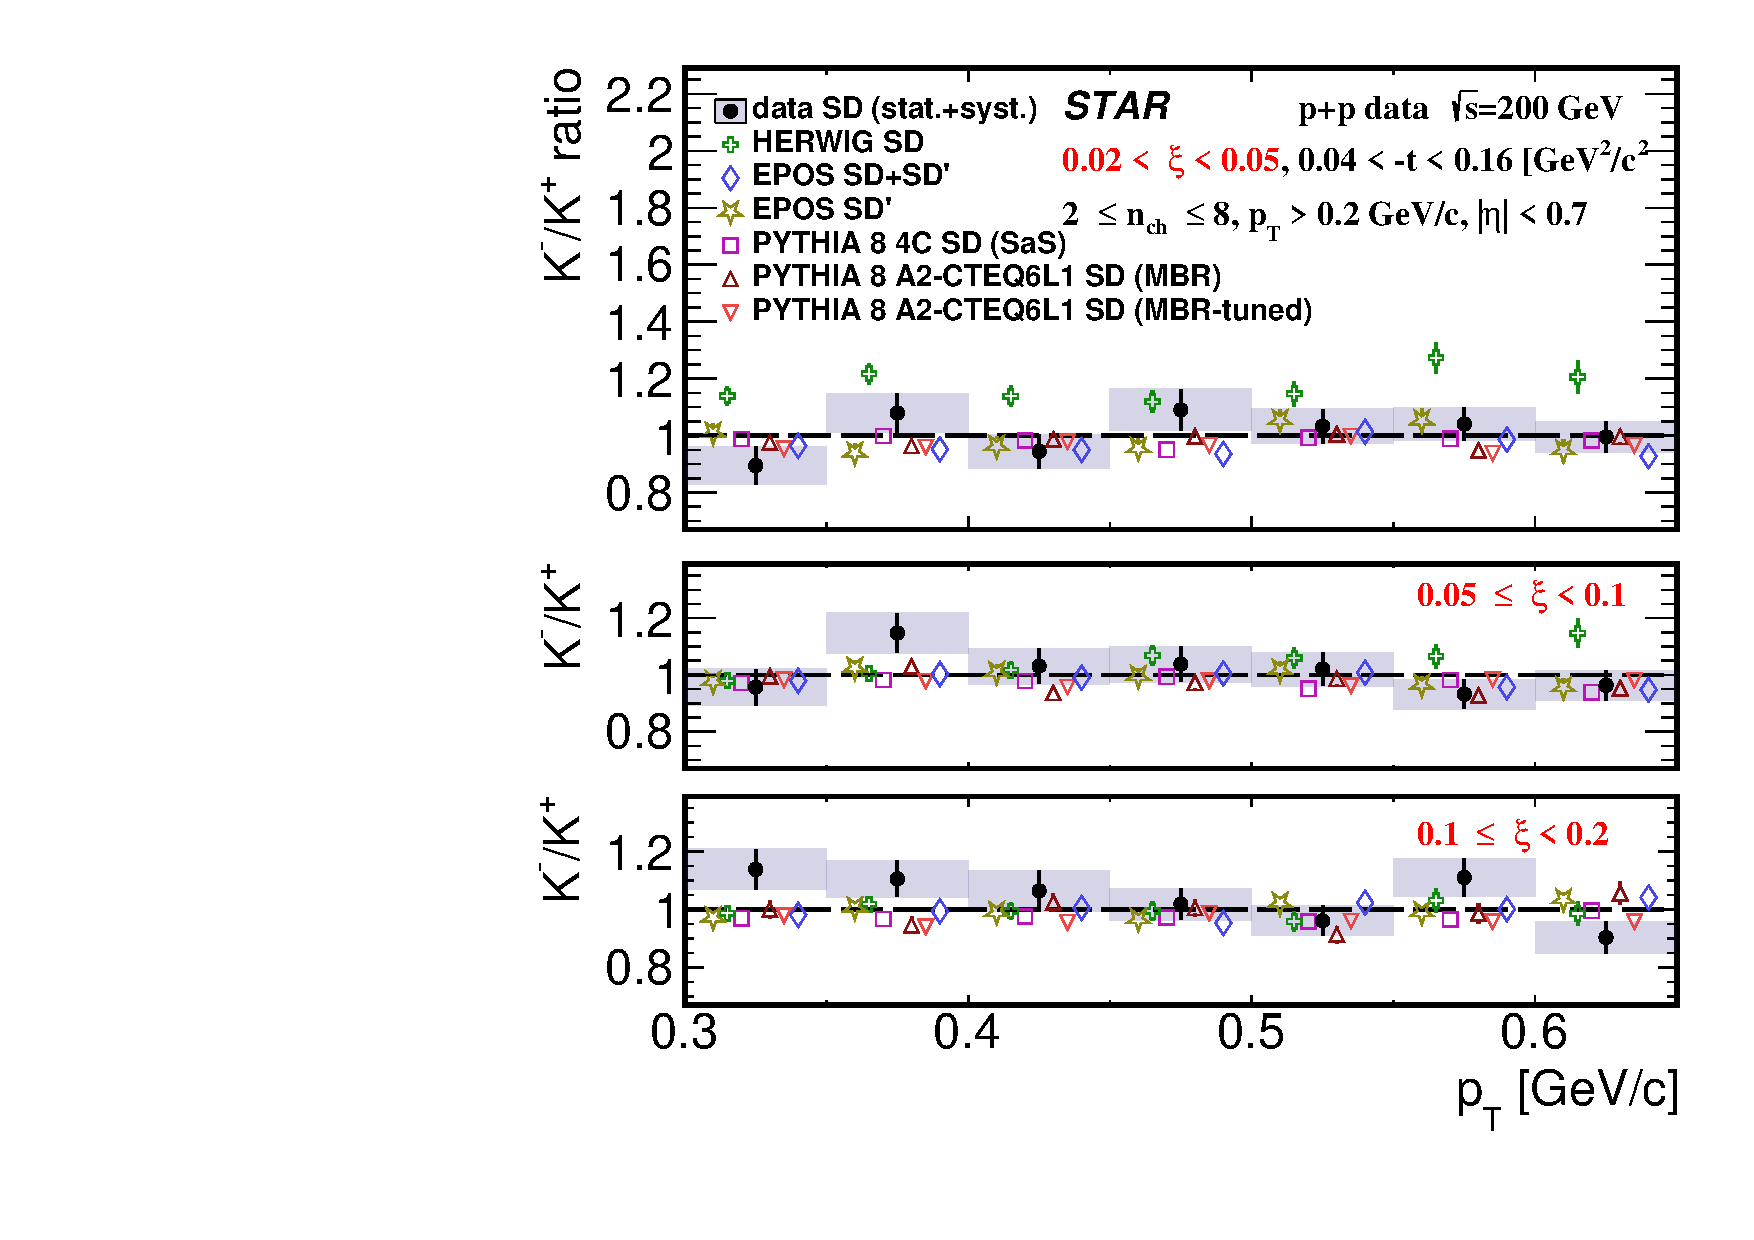
\includegraphics[width=.99\textwidth,page=1]{chapters/chrgSTAR/img/results/particleRatio_prt_1.pdf}
	%
	\caption[Ratio of production yields of $K^-/K^+$ as a function of $p_T$ shown separately for three ranges of the $\xi$.]{Ratio of production yields of $K^-/K^+$ as a function of $p_T$ shown separately for three ranges of the $\xi$: (top) $0.02<\xi<0.05$, (middle) $0.05<\xi<0.1$, (bottom) $0.1<\xi<0.2$.}
	\label{results_star_kaon}
	
\end{figure}

\begin{figure}[bh]
	\centering
	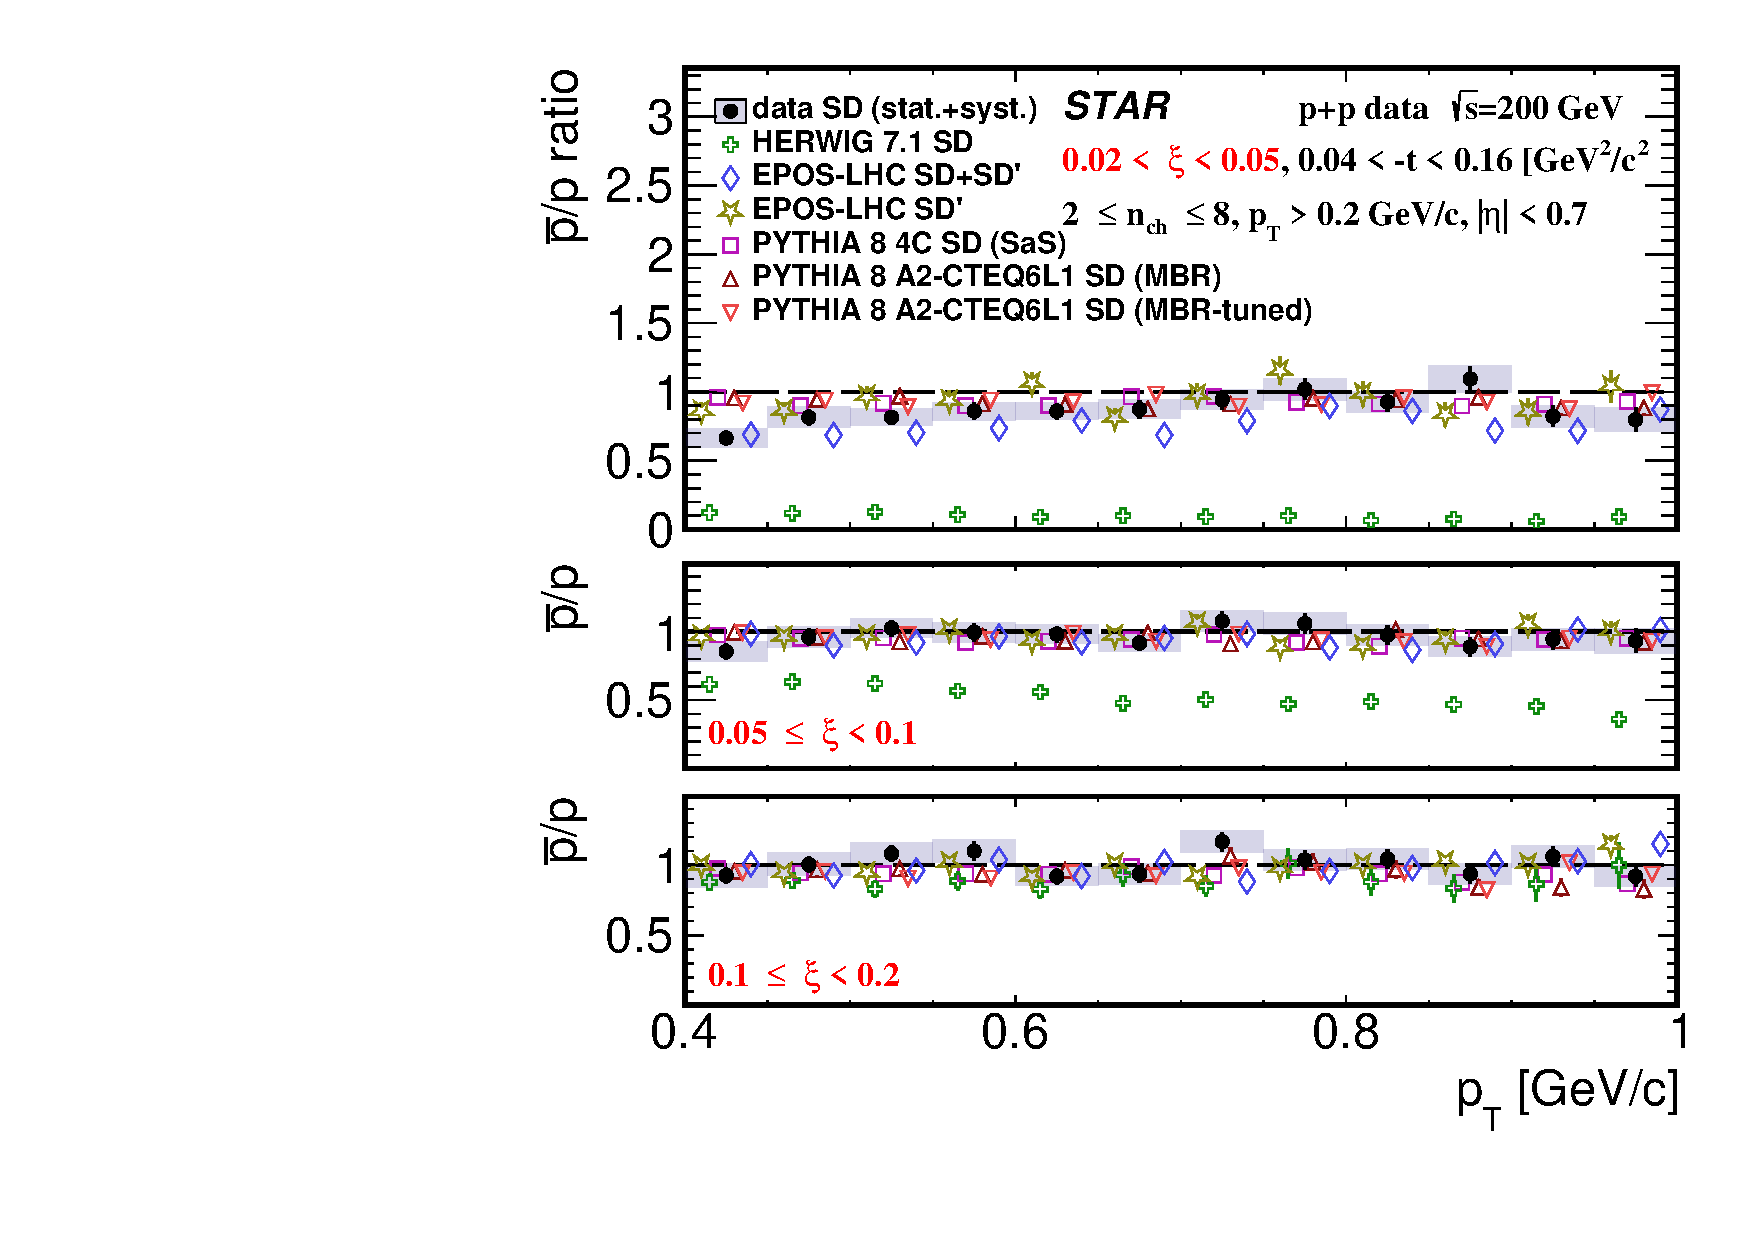
\includegraphics[width=.99\textwidth,page=1]{chapters/chrgSTAR/img/results/particleRatio_prt_2.pdf}
	%
	\caption[Ratio of production yields of $\bar{p}/p$ as a function of $p_T$ shown separately for three ranges of the $\xi$.]{Ratio of production yields of $\bar{p}/p$ as a function of $p_T$ shown separately for three ranges of the $\xi$: (top) $0.02<\xi<0.05$, (middle) $0.05<\xi<0.1$, (bottom) $0.1<\xi<0.2$.}
	\label{results_star_proton}
	
\end{figure}

\begin{figure}[bh]
	\centering
	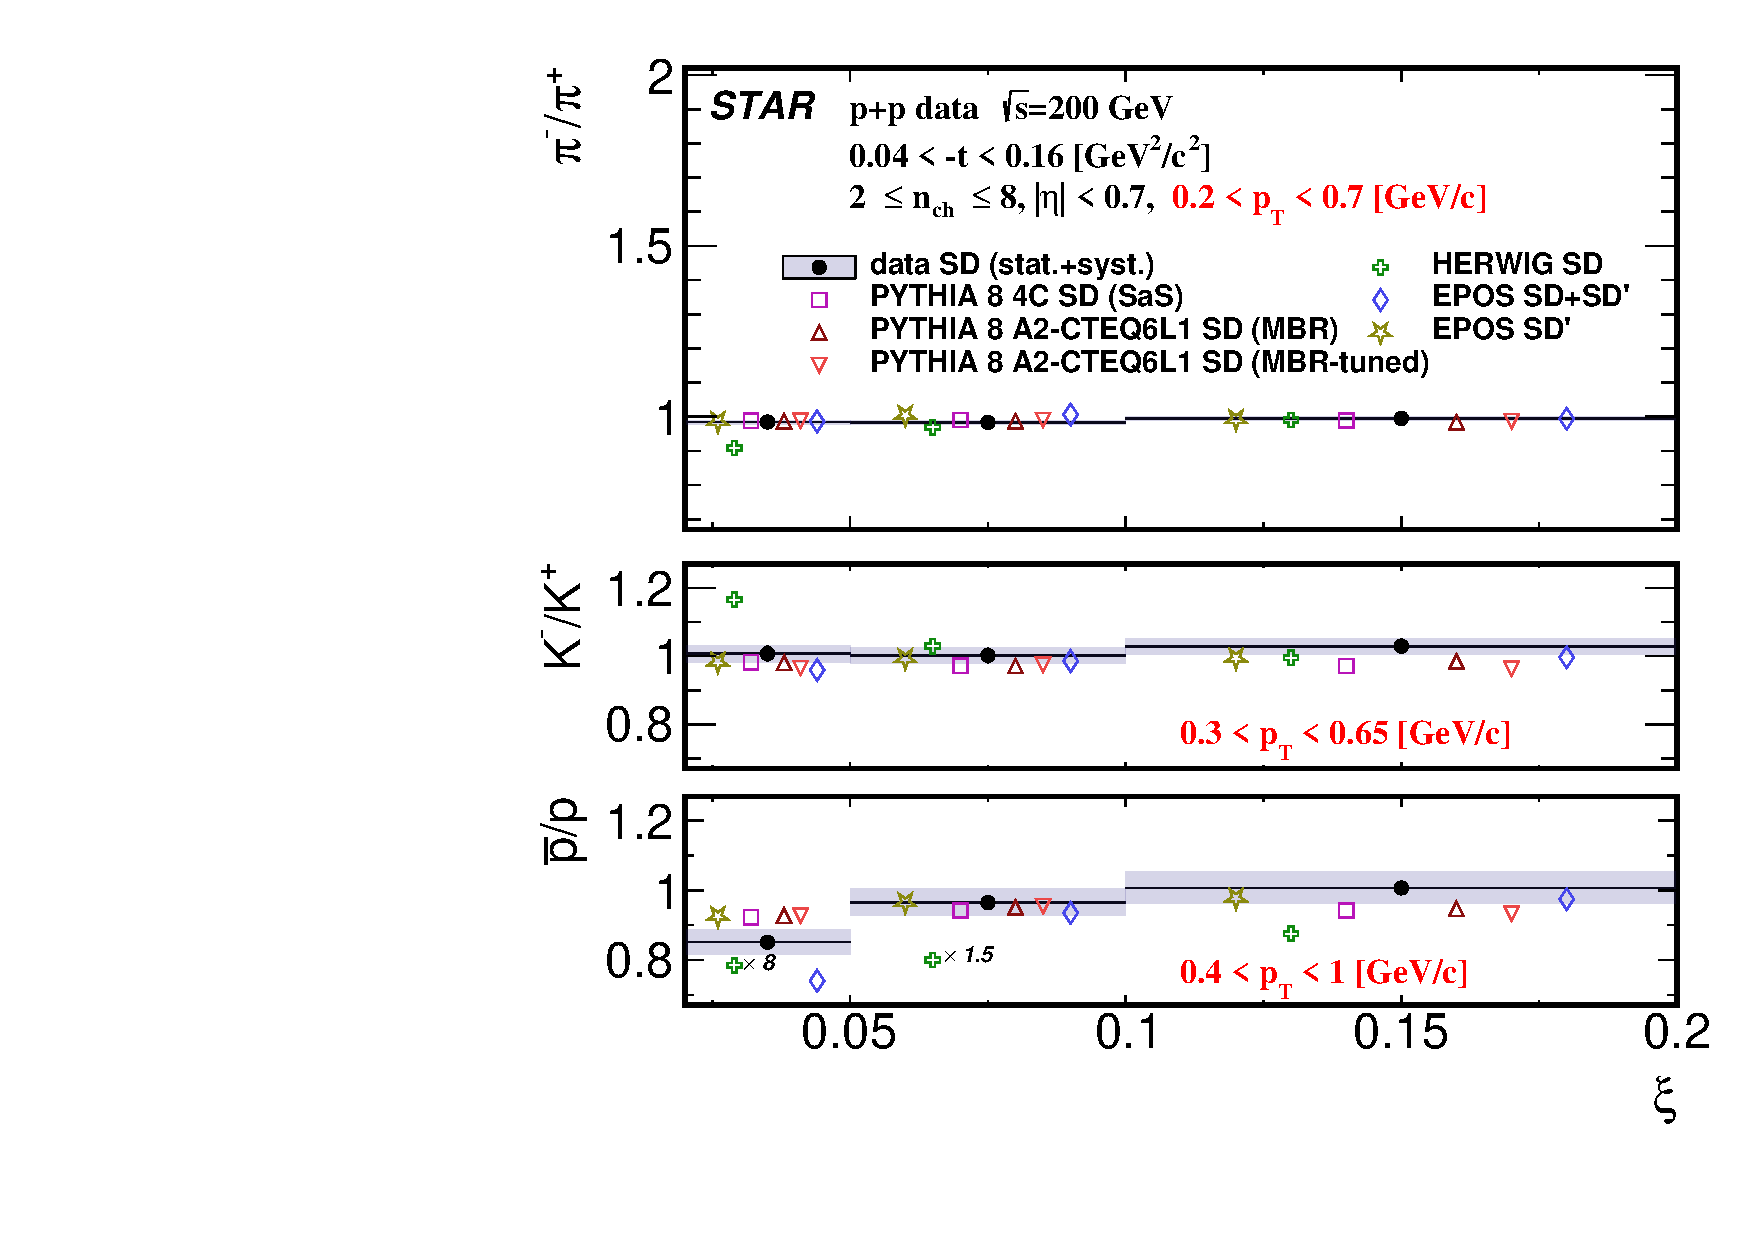
\includegraphics[width=.99\textwidth,page=1]{chapters/chrgSTAR/img/results/ratio_xi.pdf}
	%
	\caption{Ratio of production yields of $\pi^-/\pi^+$, $K^-/K^+$ and $\bar{p}/p$ as a~function of $\xi$. }
	\label{results_mean_ratio_star}
	
\end{figure}